%%%%%%%%%%%%%%%%%%% CHAPTER 1 %%%%%%%%%%%%%%%%%%%%%%%%%%%%%%%%%%%%%
%%%%%%% INTRODUCTION %%%%%%%%%%%%%%%%%%%%%%%%%%%%%%%%%%%%%%%%%%%%%%%
\section{Introduction and Getting Started}
In the 1990s Civil Engineering programs reduced programming courses in a effort to recover hours for other topics -- a logical decision at the time, but with some consequences.  
The philosophy was that engineers would not need to be able to write computer programs, but instead just use them.  
Microsoft Excel and Lotus 1-2-3 were the dominant spreadsheet software programs (Borland QuatroPro was a close third), and with macro instruction capability, much legitimate engineering computation could be performed within these tools.  
In fact I developed Excel spreadsheets that could solve multi-dimensional diffusion problems (3D groundwater flow) using fully implicit finite difference methods.  These spreadsheets were slow relative to MODFLOW, but you could watch the solutions evolve -- ultimately the process was deemed a waste, because of the ever present ``... there is no longer a need for engineers to be able to write programs.''
Later on I developed spreadsheets to perform pressurized pipe network simulation, gradually varied flow simulation, and rudimentary water-hammer and St-Venant equation solutions.  The spreadsheets were never really practical (yes they worked well, produced the same results as professional products, but were always intended a pedagogical tools), but they proved an important point -- if you could teach a computer to follow an algorithm it made you a more self-help user of the professional tools.

In 2014 several of my students expressed desire to understand programming -- they all know how to write code, but feel they don't know how to build algorithms (and implement them).   This workbook is an attempt to remedy that student self-identified weakness.   I conducted several one-to-one classes (as special topics); they learned a lot, I learned even more.  This book is a tribute to their interests.

The workbook plan is to introduce a programming tool -- I have selected \textbf{R} because it has a rich development environment already available, graphics is almost trivial, then apply that tool to selected hydraulics problems of practical value.  In the end the reader ends up with a toolkit that can either stand-alone, or more likely supplement professional tools they will eventually use.

 \textbf{R} is freeware, but it is built and maintained by a consortium of programmers and statisticians.  They have evolved the environment to work on most of the main architectures (MacOS, Windows, Linux); there are even parallel processor and GPU builds available, and a company called RStudio provides the APIs to even run it server side.  Much of the underlying code is C, C++, and well proven FORTRAN routines.
%%%%%%%%%%%%%%%%%%%%%%% CHAPTER 2 %%%%%%%%%%%%%%%%%%%%%%%%%%%%%%%
%%%%%% Getting Started %%%%%%%%%%%%%%%%%%%%%%%%%%%%%%%%%%%%%%%%%%%%%%%
\subsection{About \textbf{R}}
\textbf{R} is a open source envrionment that runs on Windows, Linux/UNIX, and Mac OS X.  The individual binaries are unique to each OS and architecture, but \textbf{R} ``source'' is interchangeable among machines.  With very minor differences, an \textbf{R} script will run equally well on any machine.

\textbf{R} is a statistical analysis tool, it is also a programming tool and language, it is also a nearly ``publication'' quality graphics tool.  Naturally all this capability comes at a cost (especially since the software is distributed for ``free'') --- learning to do more than simple calculations takes some time (not much), but the skill is highly perishable.  You will need to keep notes, or copies of your \textbf{R} scripts for future reference.  Relearning after some time away from \textbf{R} is pretty simple, so the modeler only has to pay the steep learning cost once.

The remainder of this essay shows how to obtain and install \textbf{R} on a Windows machine.  Macintosh and Linux installs are accomplished in a similar fashion.  For the truly insane, the entire envrionment can be built from source on any machine with PERL, gcc, and gfortran compliers (default in Linux, easy to obtain for other architectures).

\subsection{Getting Started}
The first step required (for using \textbf{R} as a programming tool) is to install \textbf{R} on your computer.
The source of the binary builds is the same regardless of the underlying operating system -- the Comprehensive R Archive Network (CRAN for short).
The remainder of this chapter shows how to get the tool running on the three main operating systems in current practice.
\subsubsection{Windows Users}
The purpose of this section is to demonstrate how to get \textbf{R} running on a Windows computer.  This document assumes the following:
\begin{enumerate}
\item You have internet connection.
\item You have sufficient user privileges to install software on your machine.  (If you need someone else to install, I did my install by running the installer as a local administrator --- obviously you need the password)
\item You have 60MB or so of vacant disk space on the system directory.
\end{enumerate}

The step-by-step guide is presented as a series of screen captures.  Obviously adjust inputs to fit your machine.  The version in these screen captures is quite dated --- use the most recent, stable version offered on CRAN (Comprehensive R Archive Network).\footnote{I have updated the screen captures for Windows 10 --- so these should replicate the steps.}

%\section*{}

\begin{figure}[h!] %  figure placement: here, top, bottom, or page
   \centering
   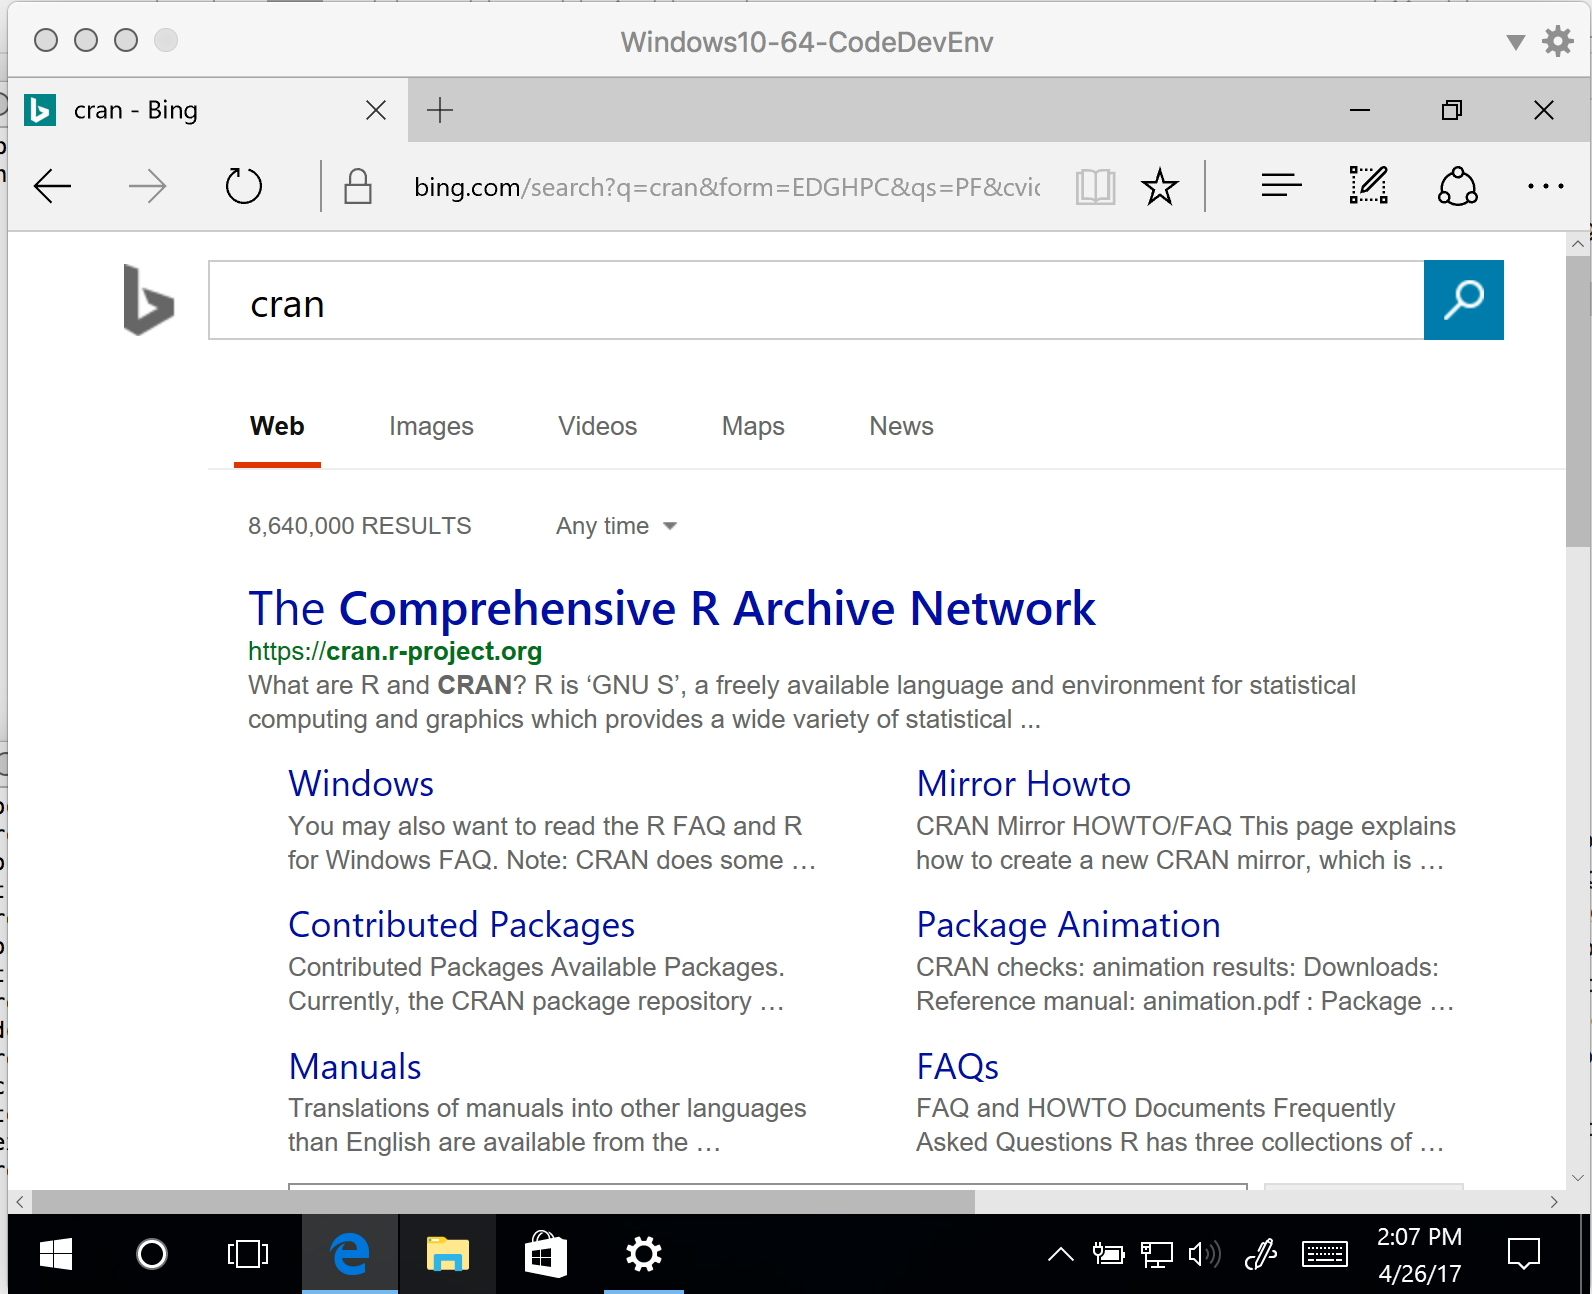
\includegraphics[width=4.5in]{./1-Introduction/googleR.jpg} 
   \caption{Google ``R'' (alternatively google CRAN)}
%   \label{fig:example}
\end{figure}

\begin{figure}[h!] %  figure placement: here, top, bottom, or page
   \centering
   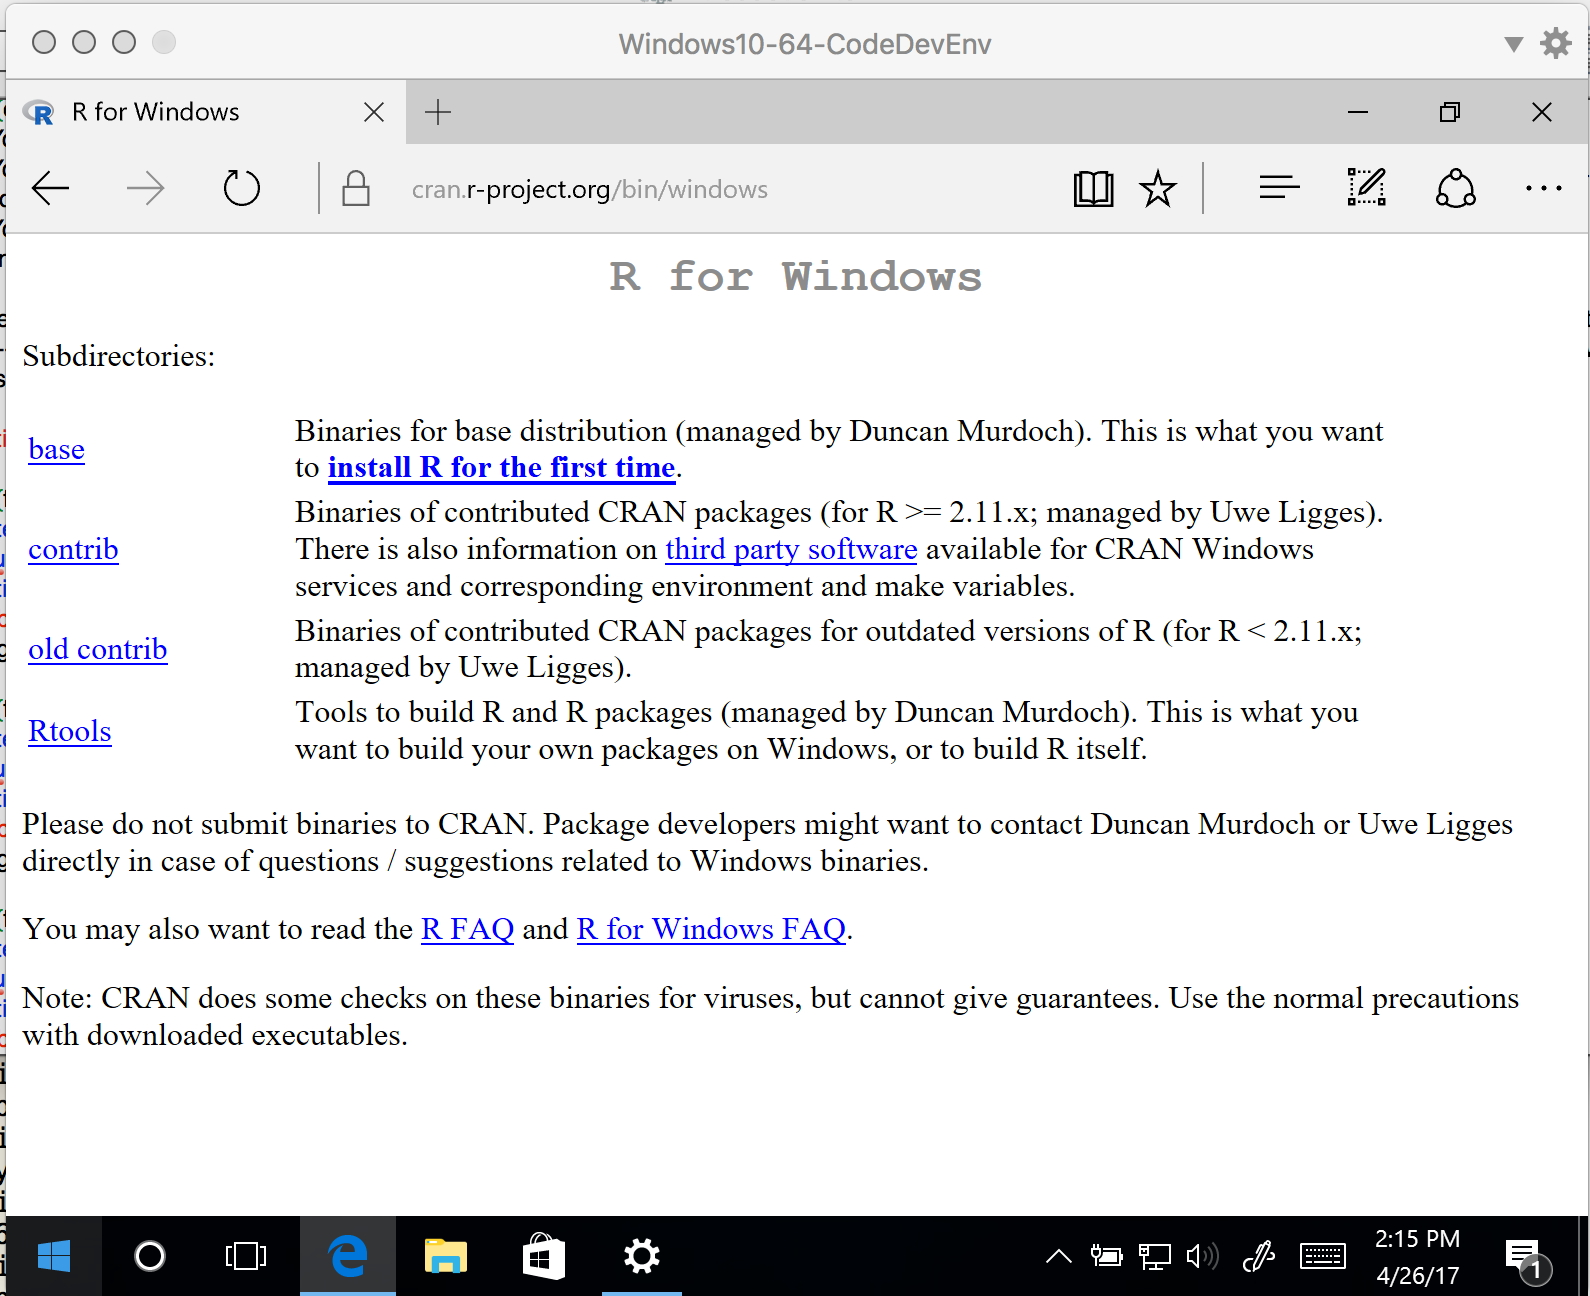
\includegraphics[width=4.5in]{./1-Introduction/gnuRproject.jpg} 
   \caption{Taking the ``Windows Link''}
%   \label{fig:example}
\end{figure}

\begin{figure}[h!] %  figure placement: here, top, bottom, or page
   \centering
   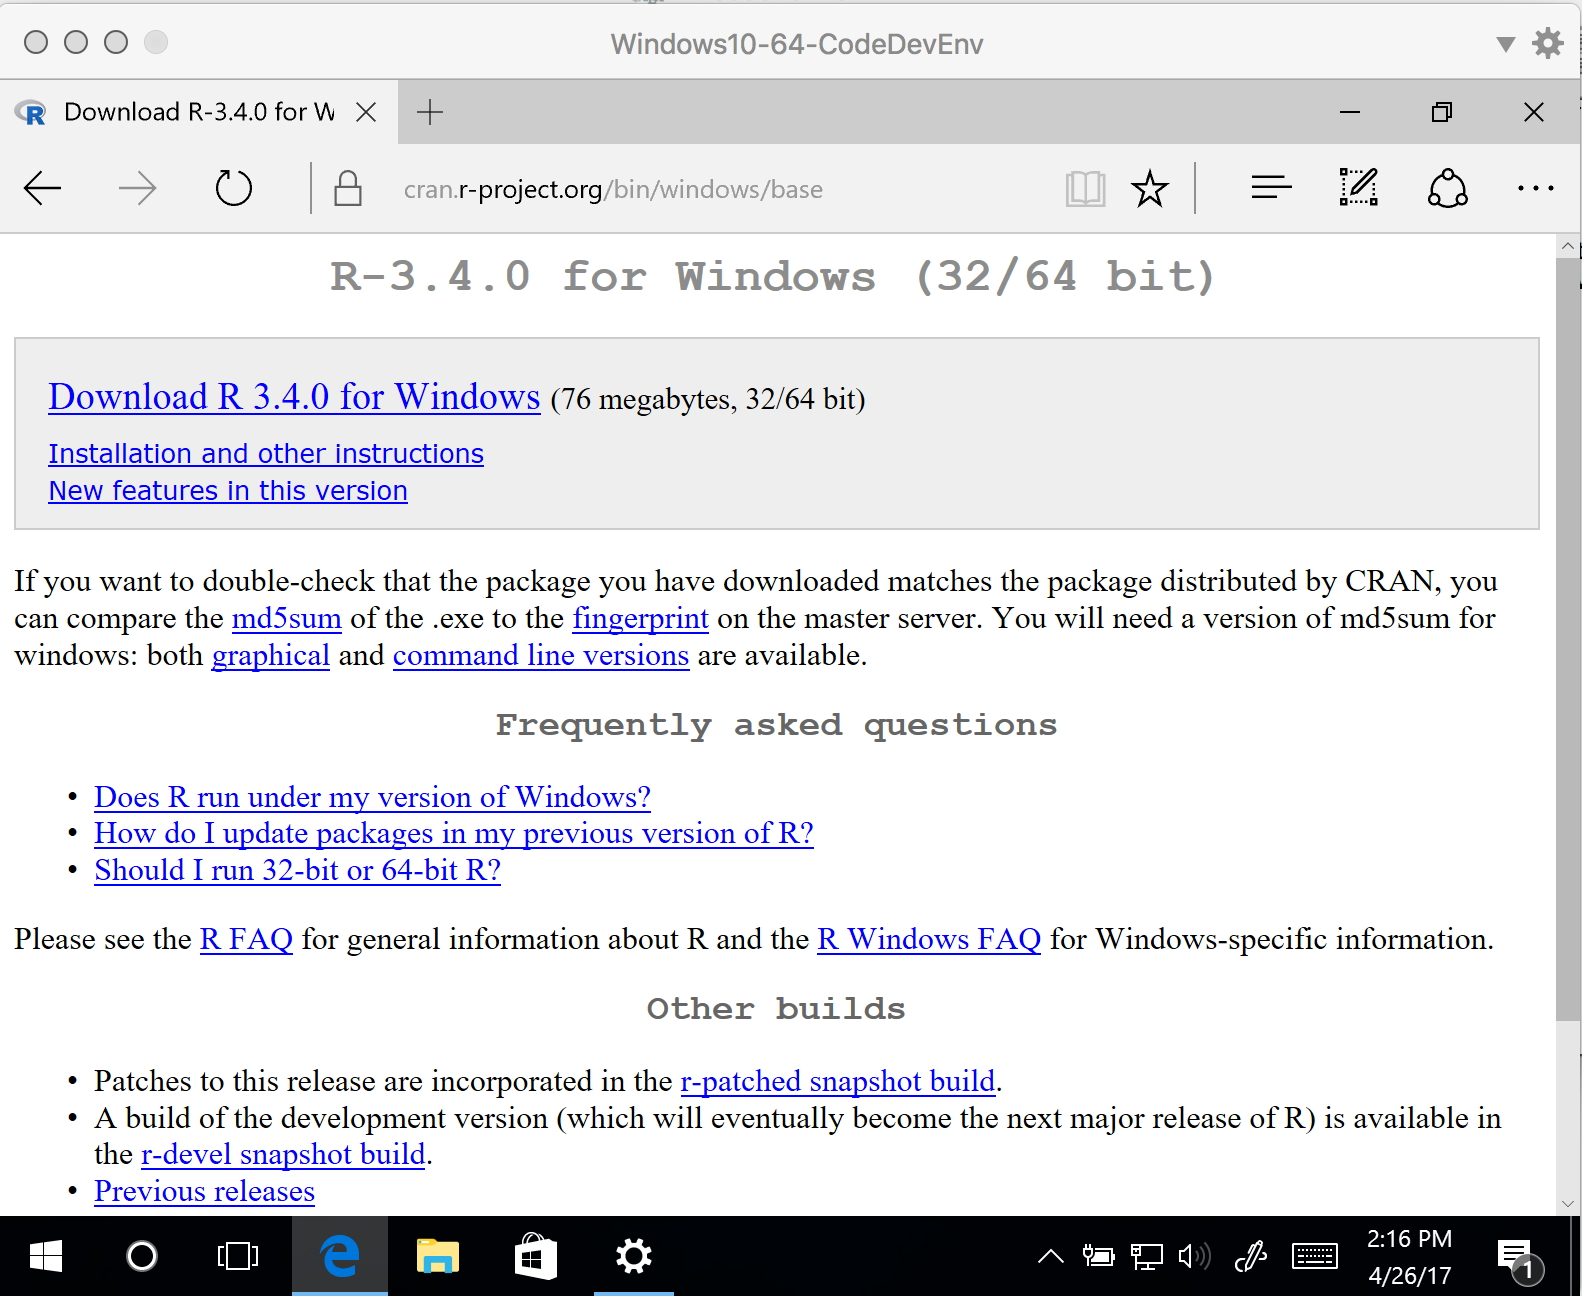
\includegraphics[width=4.5in]{./1-Introduction/downloadR.jpg} 
   \caption{Choose ``Install R for the First Time" -- goes to the download page.  We will next select ``Download R \dots'' and it should download a windows installer.  Choose ``save'' when prompted.}
%   \label{fig:example}
\end{figure}

\begin{figure}[h!] %  figure placement: here, top, bottom, or page
   \centering
   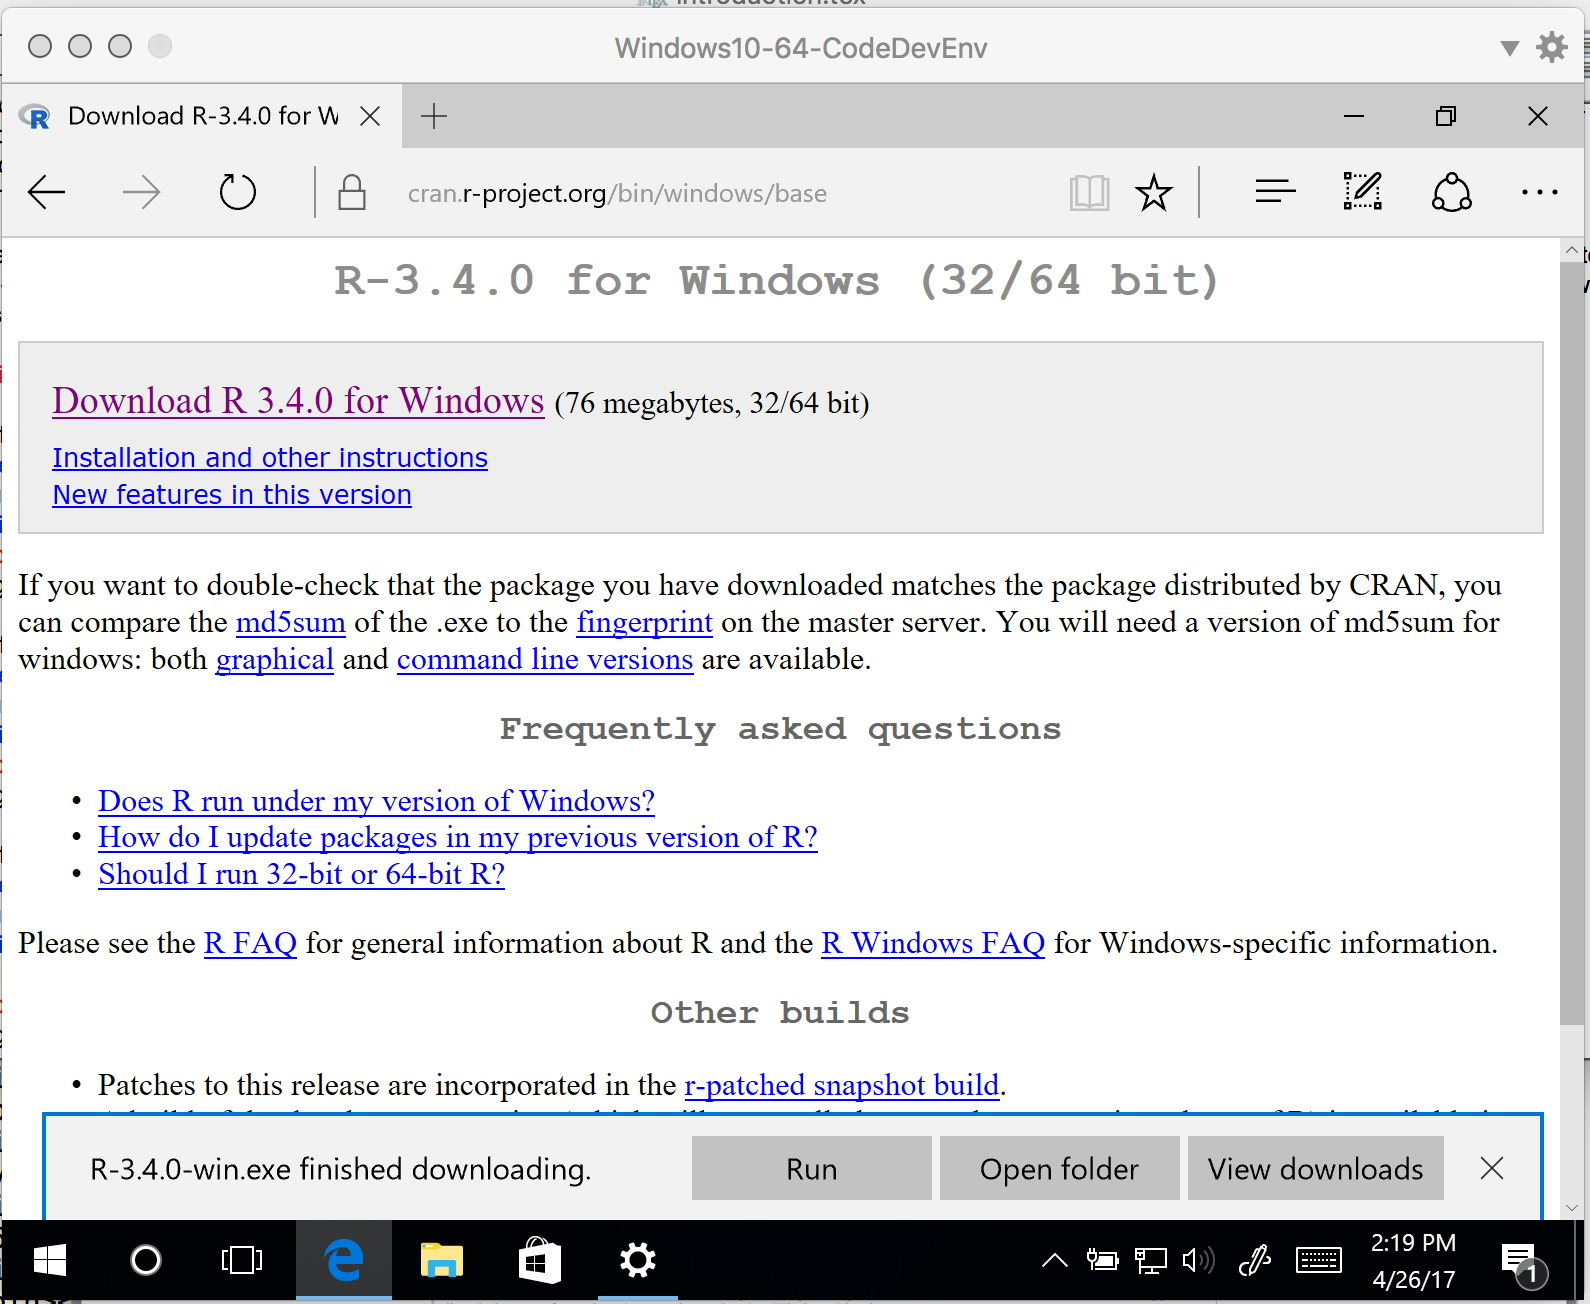
\includegraphics[width=4.5in]{./1-Introduction/repositoryR.jpg} 
   \caption{Download arrived.  Now run the installer (you need install privileges -- if its your personal laptop, then your regular user account should work). }
%   \label{fig:example}
\end{figure}

\begin{figure}[h!] %  figure placement: here, top, bottom, or page
   \centering
   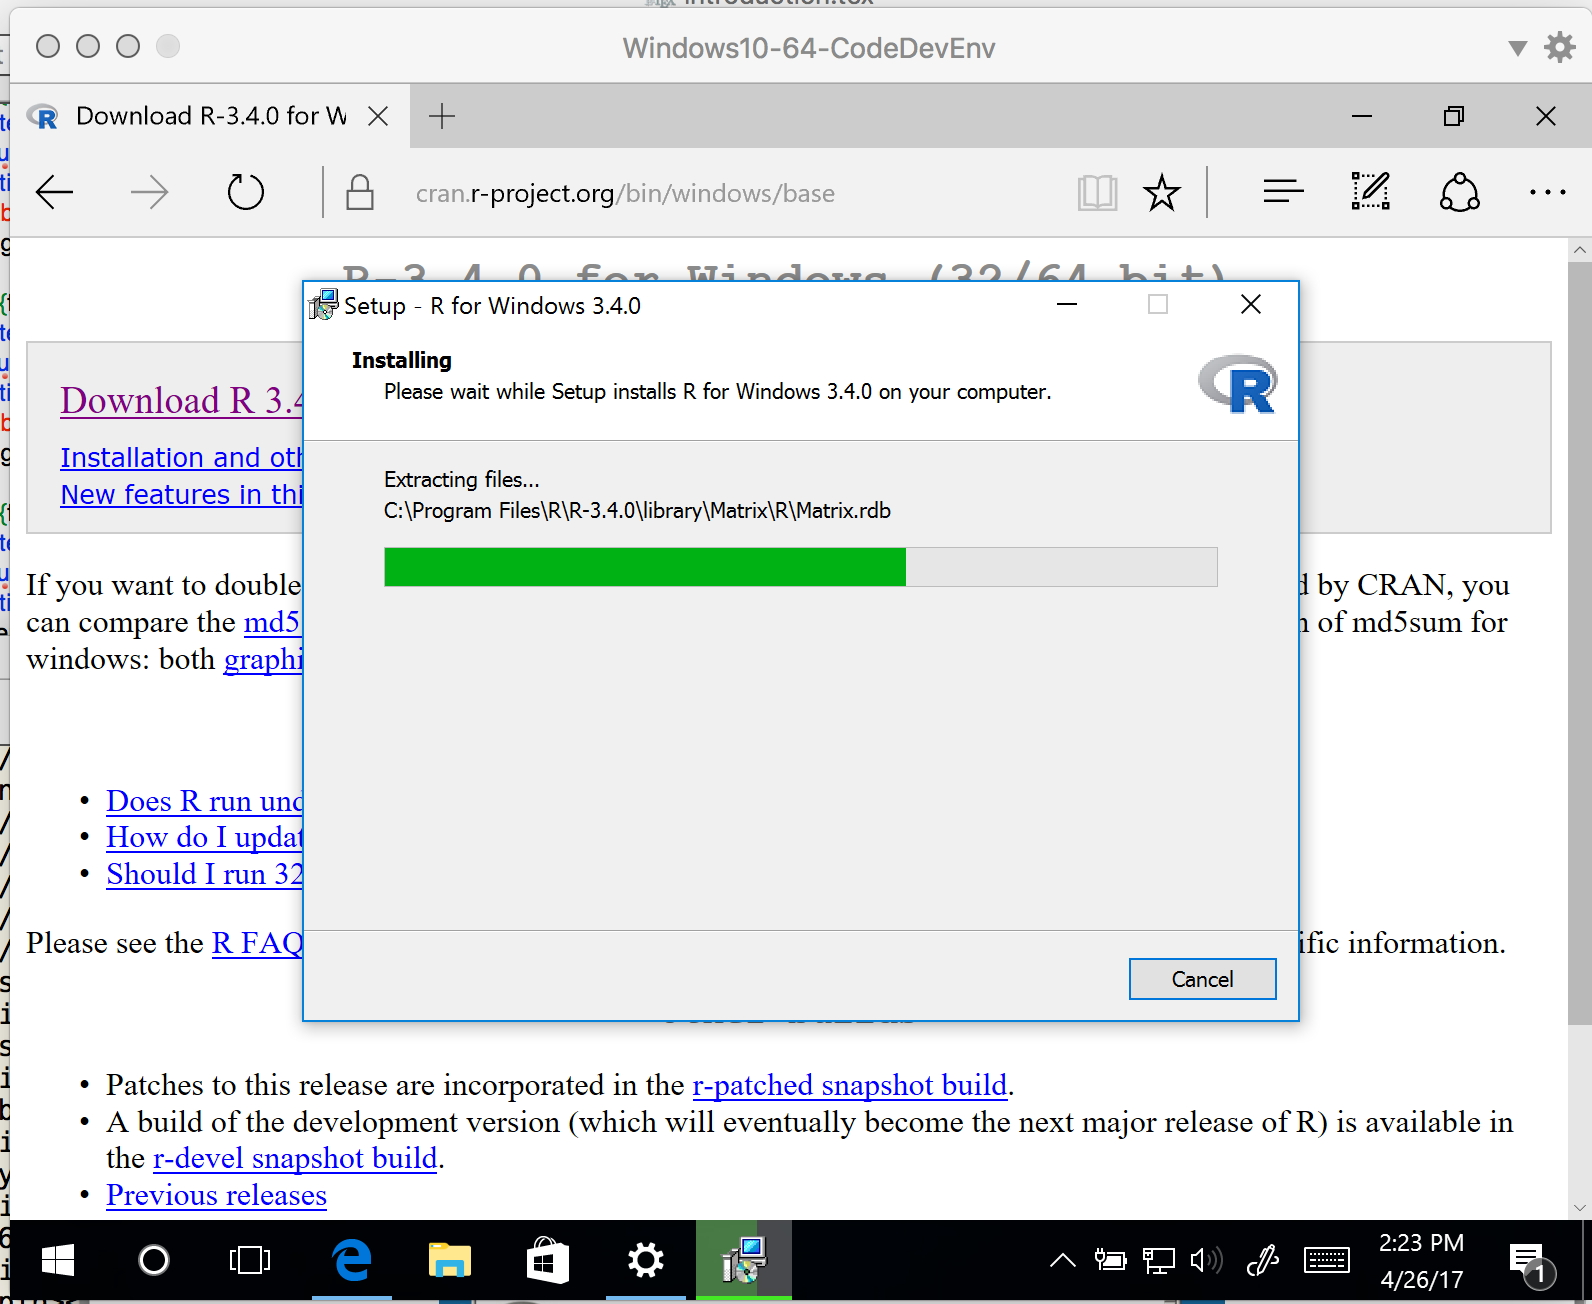
\includegraphics[width=4.5in]{./1-Introduction/chooseOS.jpg} 
   \caption{Installer run in progress.  Accept the defaults -- its just easier and works.   Later you can re-install elsewhere in your filesystem.}
%   \label{fig:example}
\end{figure}

\begin{figure}[h!] %  figure placement: here, top, bottom, or page
   \centering
   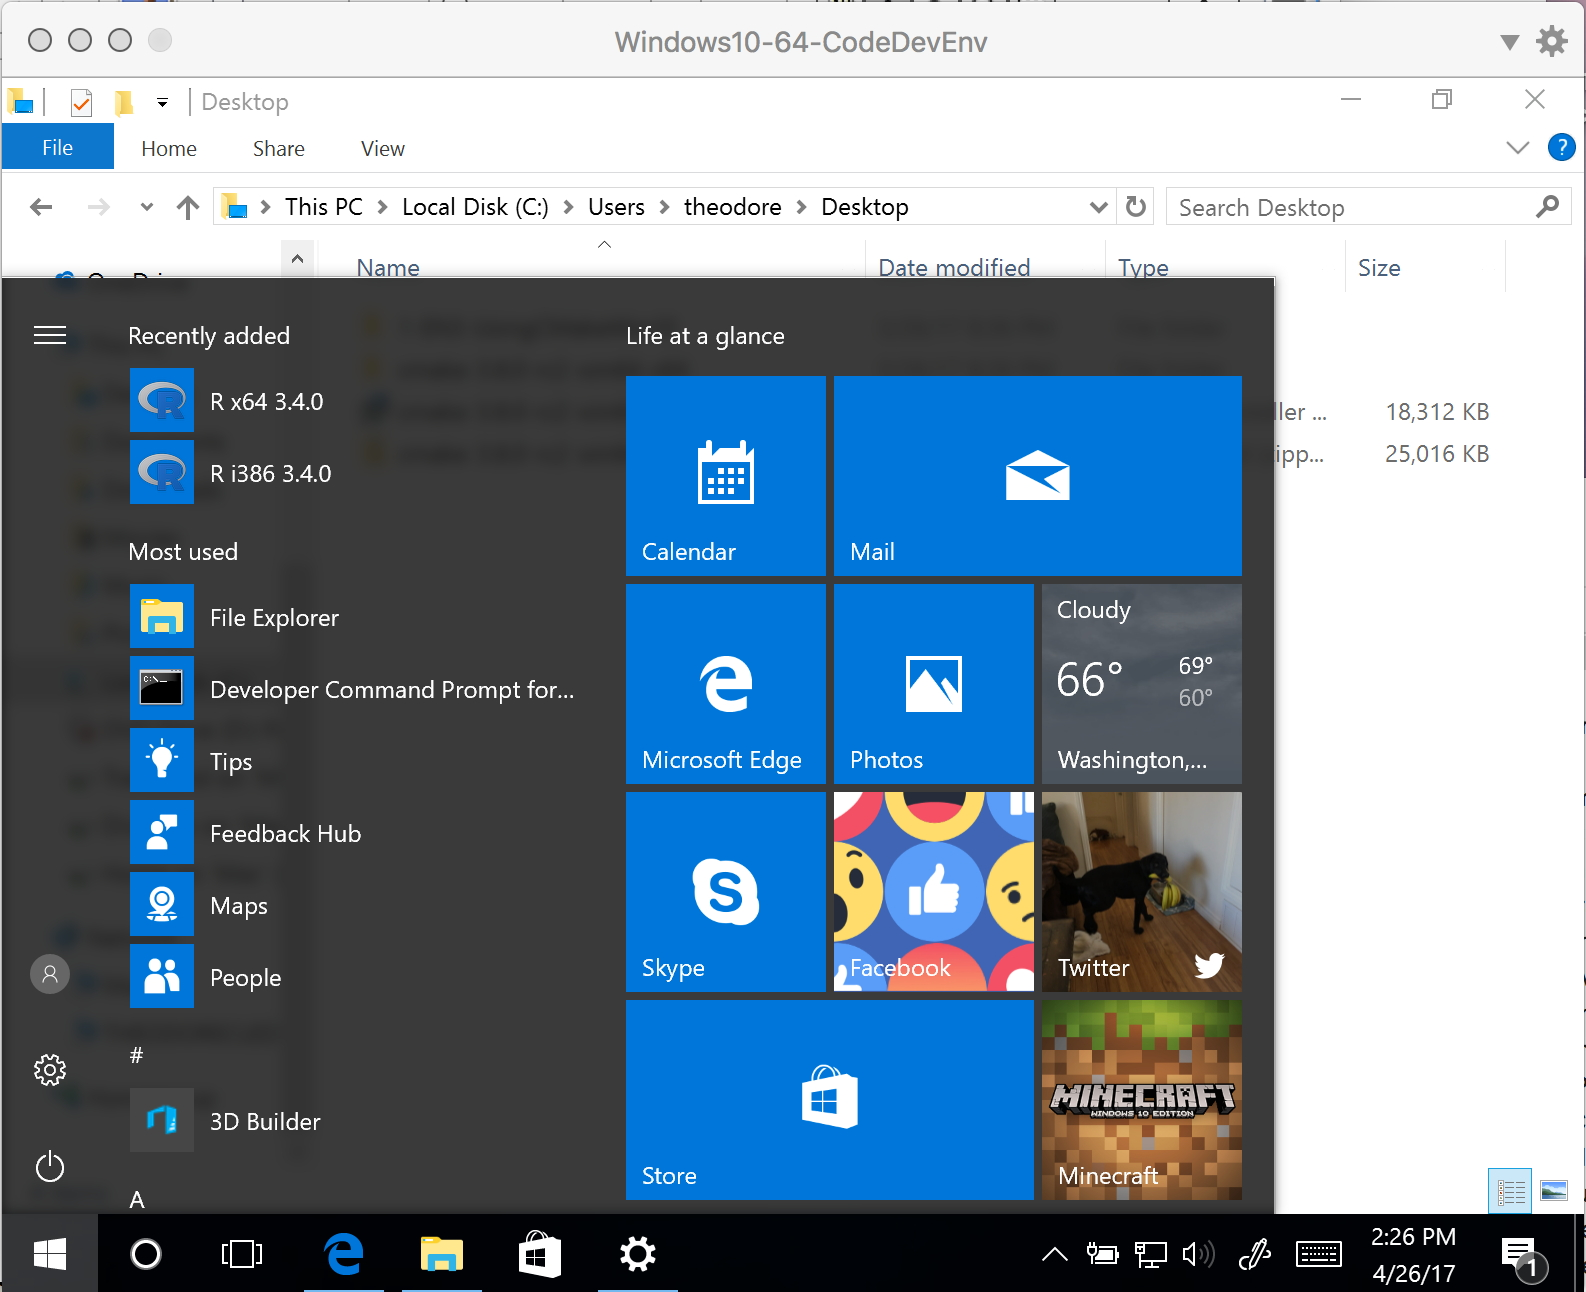
\includegraphics[width=4.5in]{./1-Introduction/baseR.jpg} 
   \caption{Installed ``R base'' packages.  Notice it installs 32-bit and 64-bit versions.  The next step is to verify the install by trying to run the program.}
%   \label{fig:example}
\end{figure}

\begin{figure}[h!] %  figure placement: here, top, bottom, or page
   \centering
   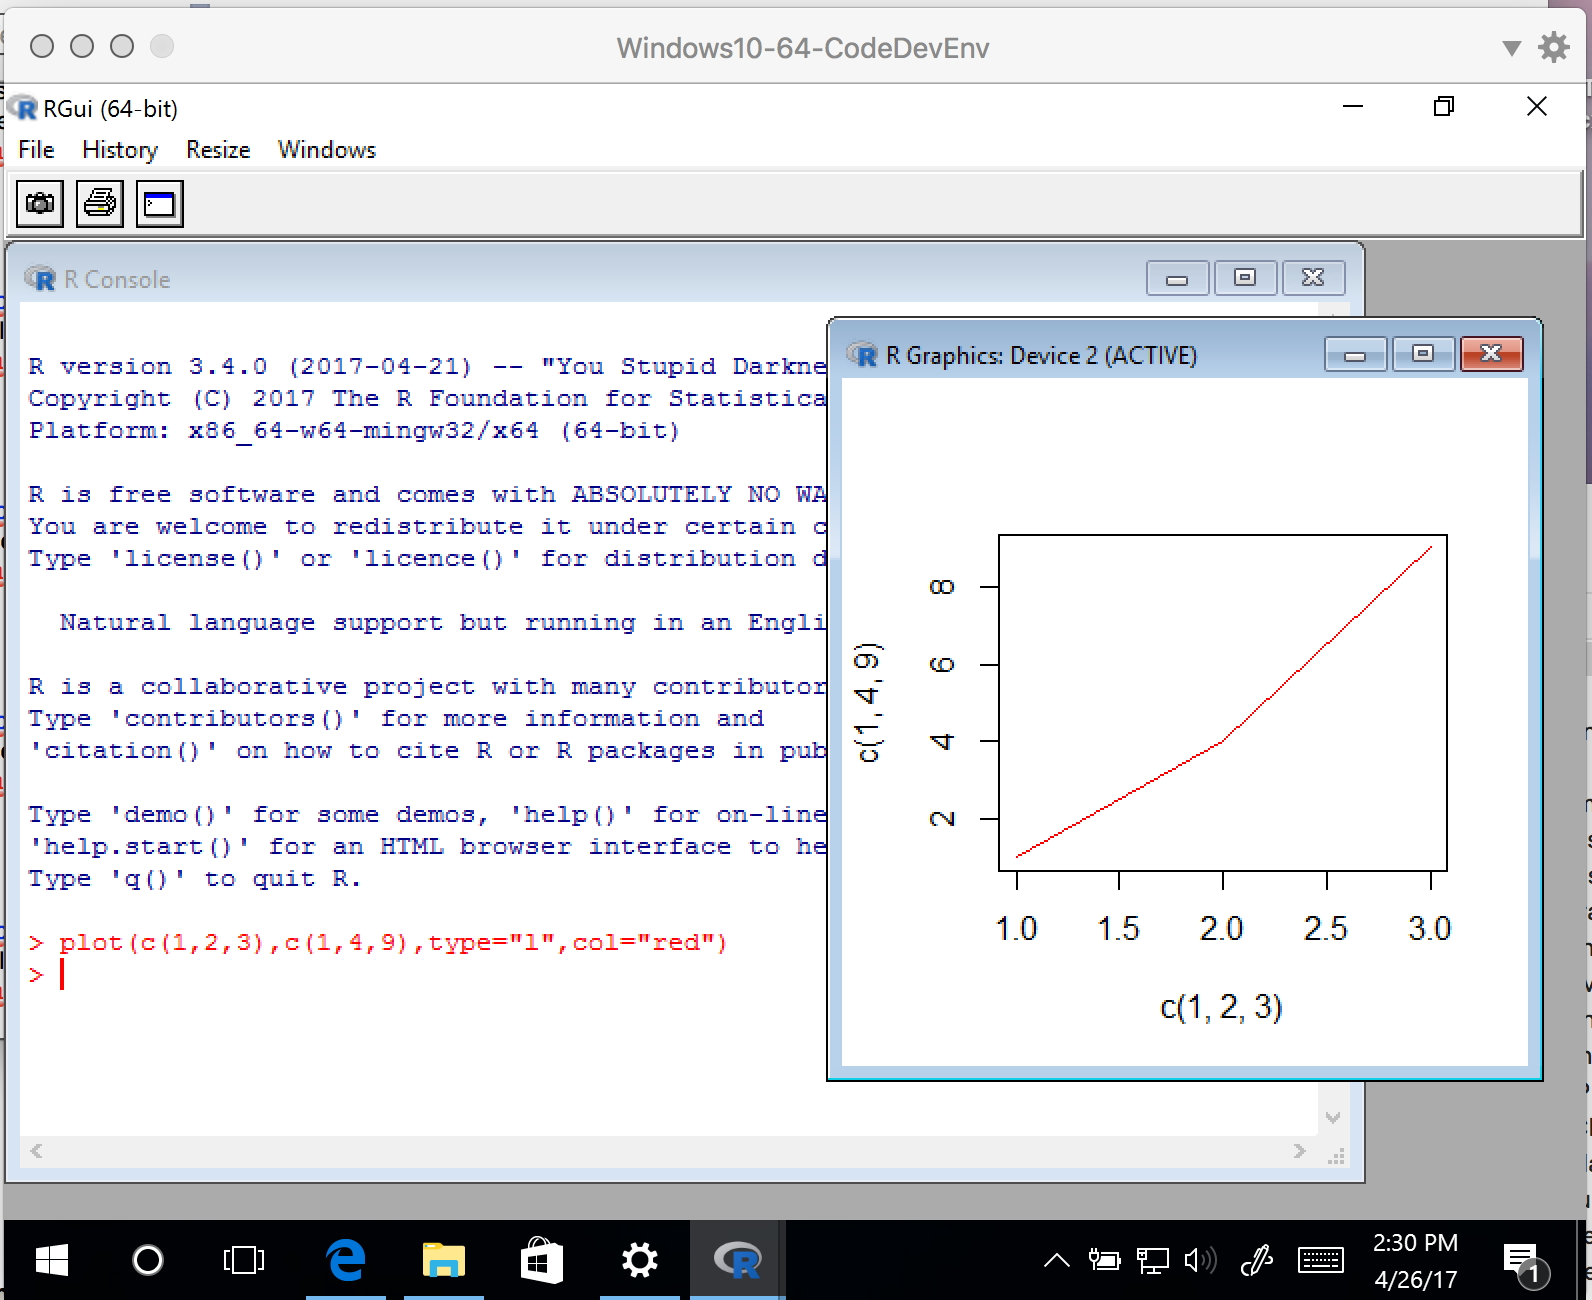
\includegraphics[width=4.5in]{./1-Introduction/installerR.jpg} 
   \caption{Run the program.  Type \texttt{plot(c(1,2,3),c(1,4,9),type="l",col="red")} into the console window.  A plot should be generated as shown.  If this works, then your install is good and now we install \textbf{R Studio}}
%   \label{fig:example}
\end{figure}

\begin{figure}[h!] %  figure placement: here, top, bottom, or page
   \centering
   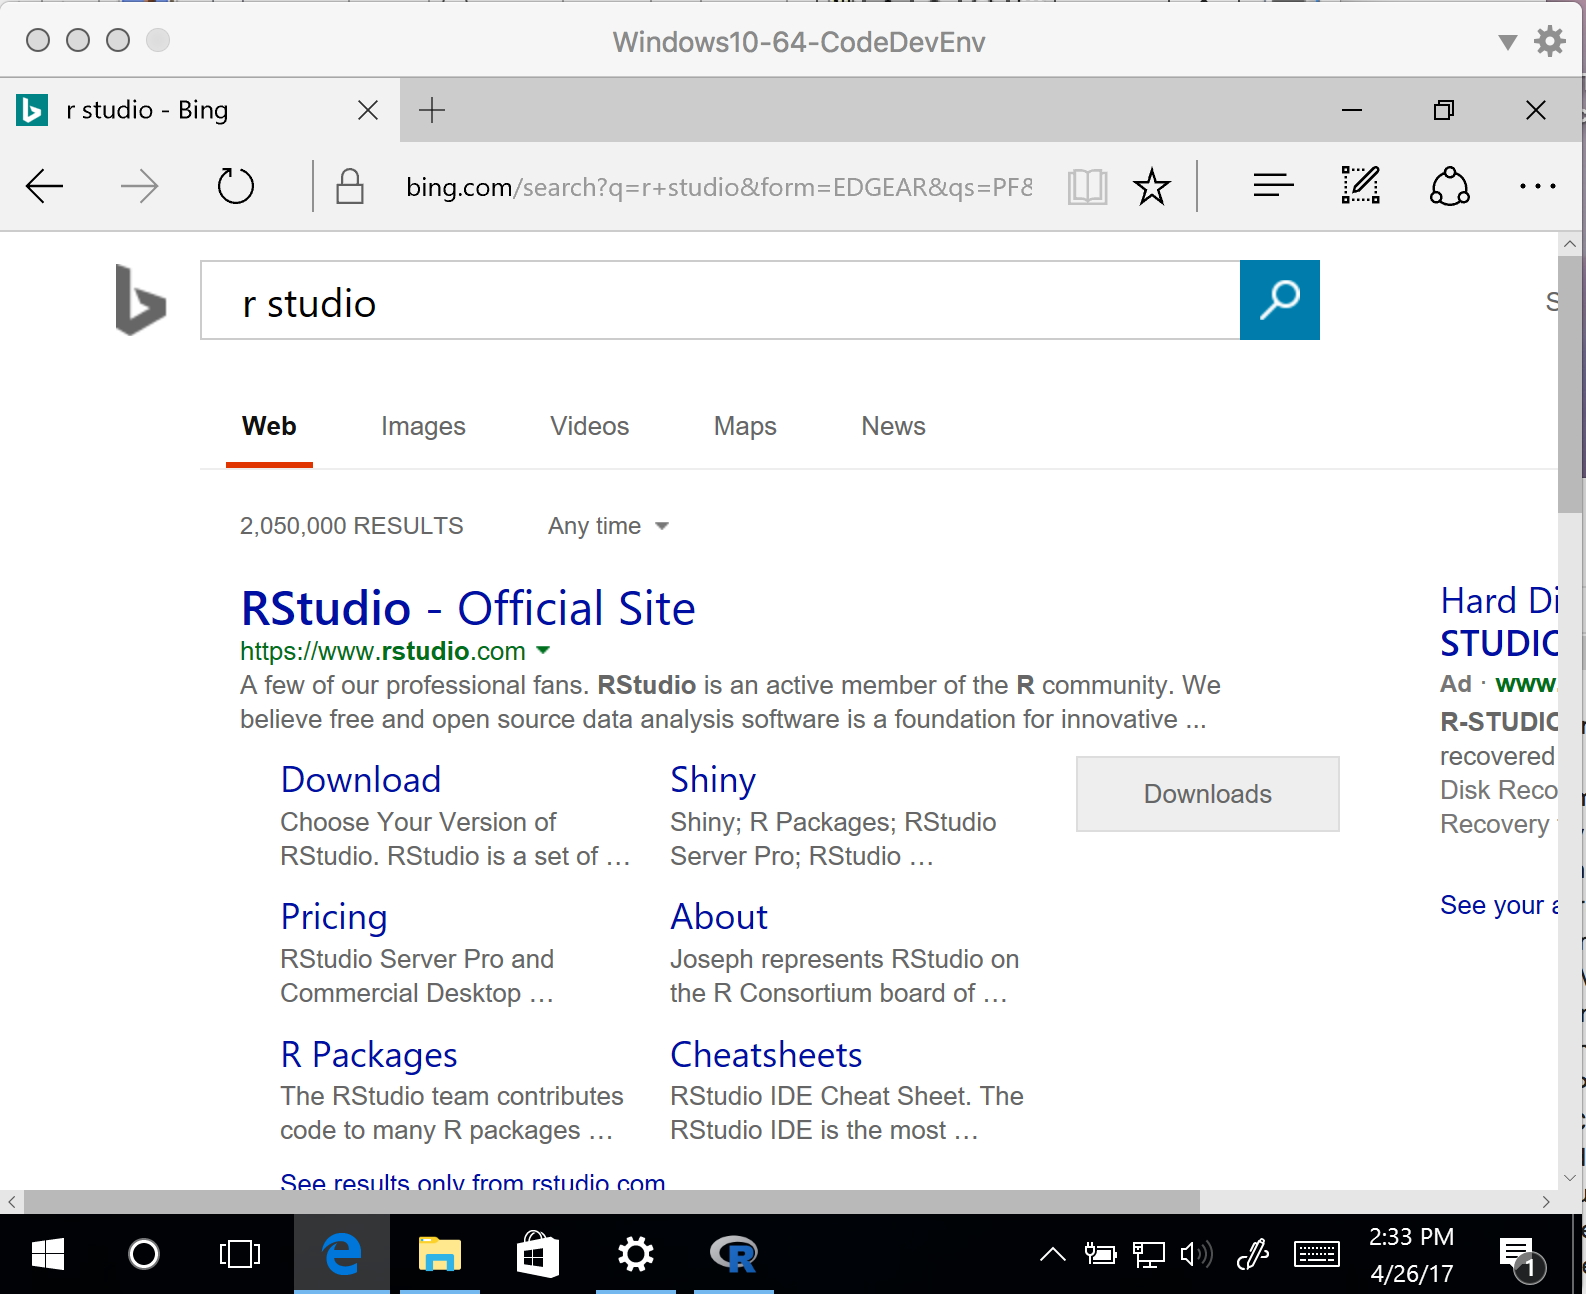
\includegraphics[width=4.5in]{./1-Introduction/downloading.jpg} 
   \caption{Search for \textbf{R Studio}.  Choose the Download link.}
%   \label{fig:example}
\end{figure}

\begin{figure}[h!] %  figure placement: here, top, bottom, or page
   \centering
   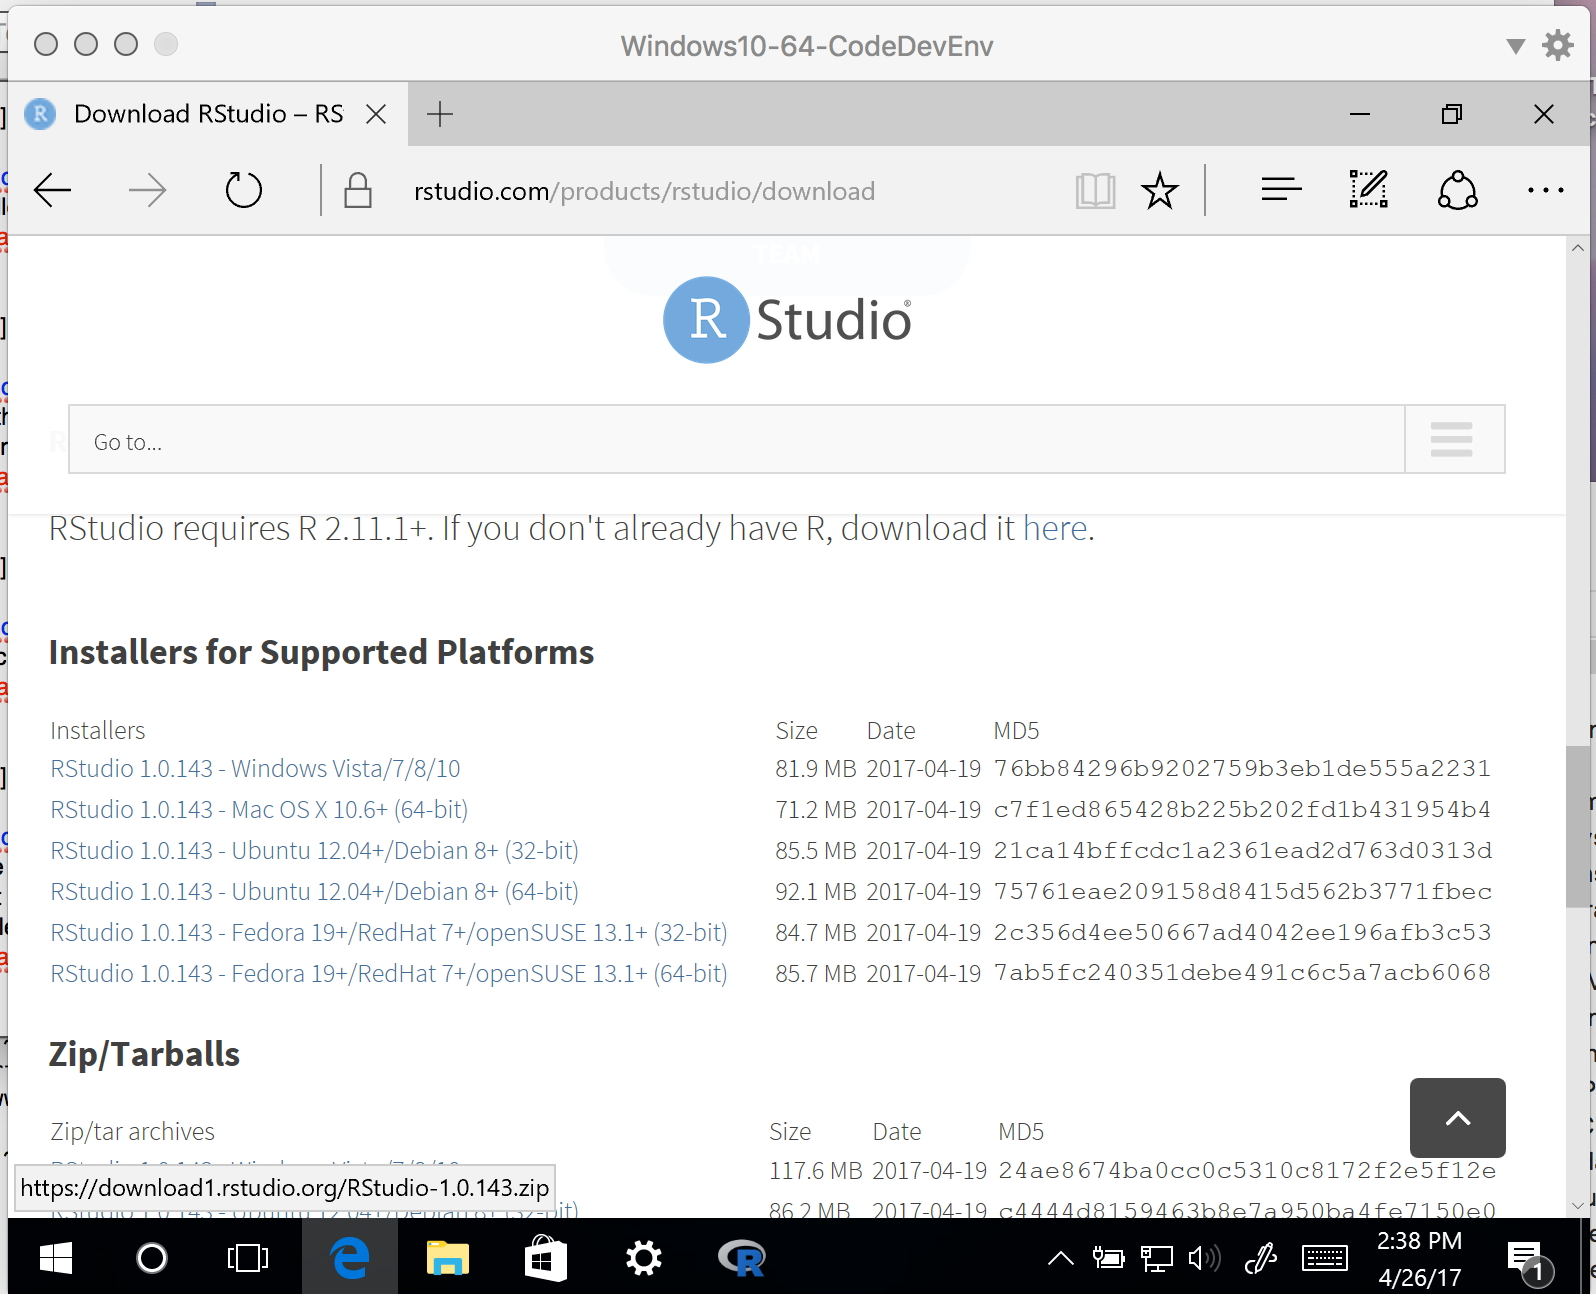
\includegraphics[width=4.5in]{./1-Introduction/runInstall.jpg} 
   \caption{In the download link scroll down to the repository.  You want to install the FREE Desktop version.  If on a windows machine, it is the top most of the installers.  Don't accidentally download the Zip/Tarballs -- all that is source code and without the compilers you cannot make much use of it.  Building from source is a challenge.  Choose the windows installer and download, select ``save'' when prompted}
%   \label{fig:example}
\end{figure}

\begin{figure}[h!] %  figure placement: here, top, bottom, or page
   \centering
   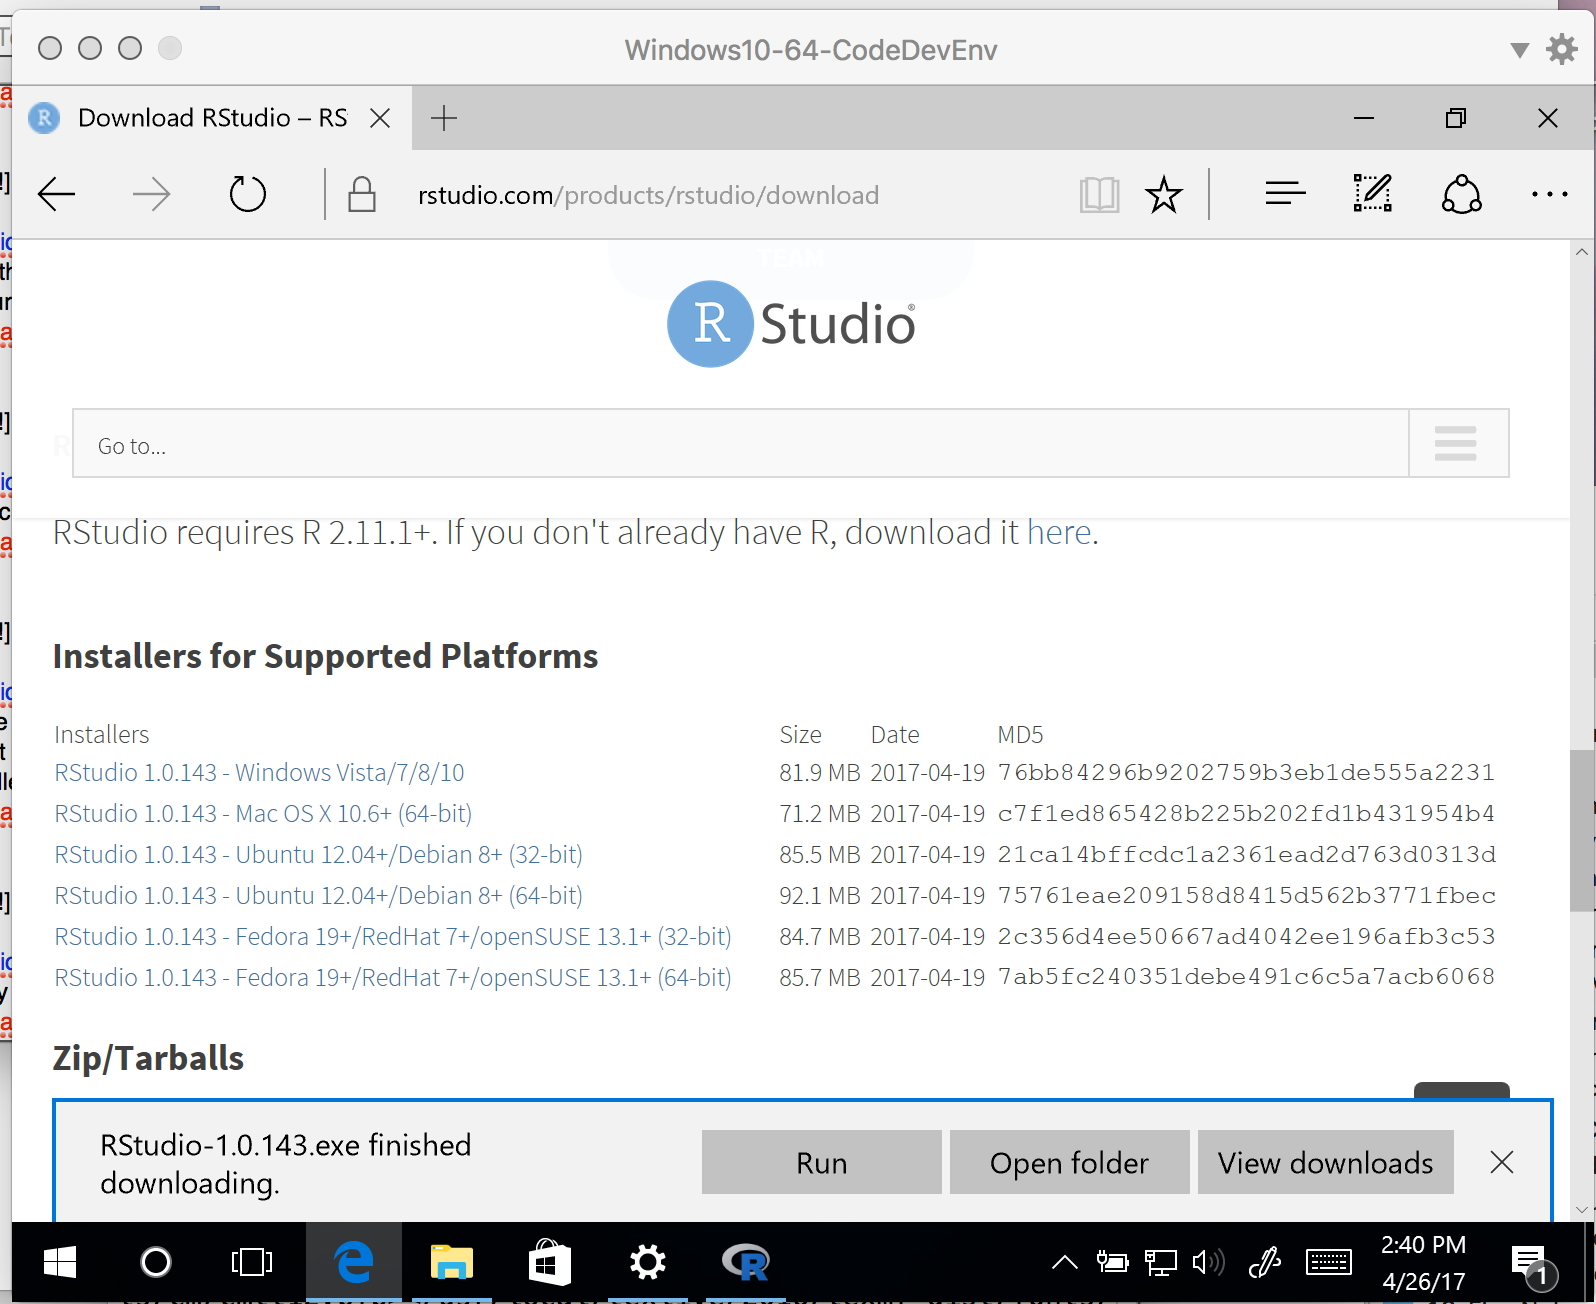
\includegraphics[width=4.5in]{./1-Introduction/repositoryR2.jpg} 
   \caption{Download arrived, run the executable (it should be a \texttt{.exe} file).  Accept the defaults during the install}
%   \label{fig:example}
\end{figure}

\begin{figure}[h!] %  figure placement: here, top, bottom, or page
   \centering
   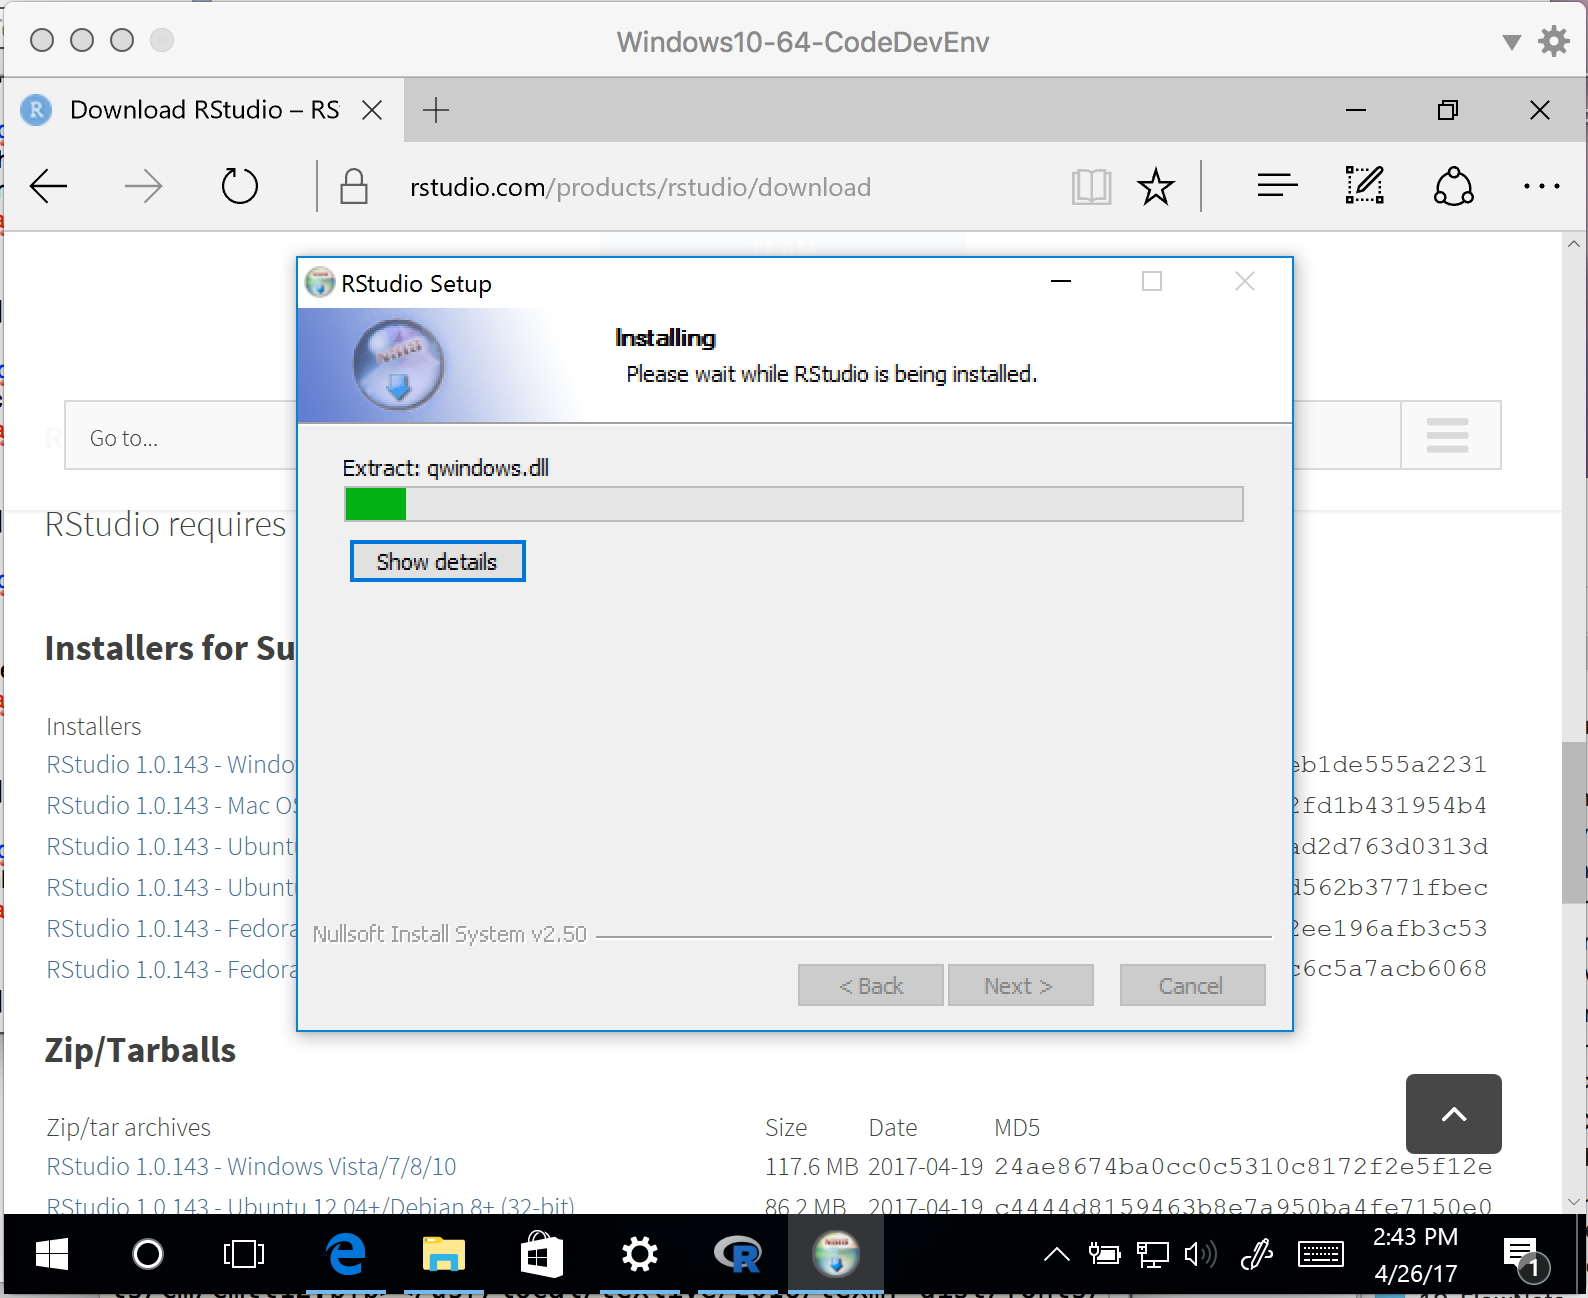
\includegraphics[width=4.5in]{./1-Introduction/runInstall2.jpg} 
   \caption{Installer in-progress.  When it completes, you should now have \textbf{R Studio} and \textbf{R} installed.  We will test the \textbf{R Studio} install using the same simple plot call}
%   \label{fig:example}
\end{figure}


\begin{figure}[h!] %  figure placement: here, top, bottom, or page
   \centering
   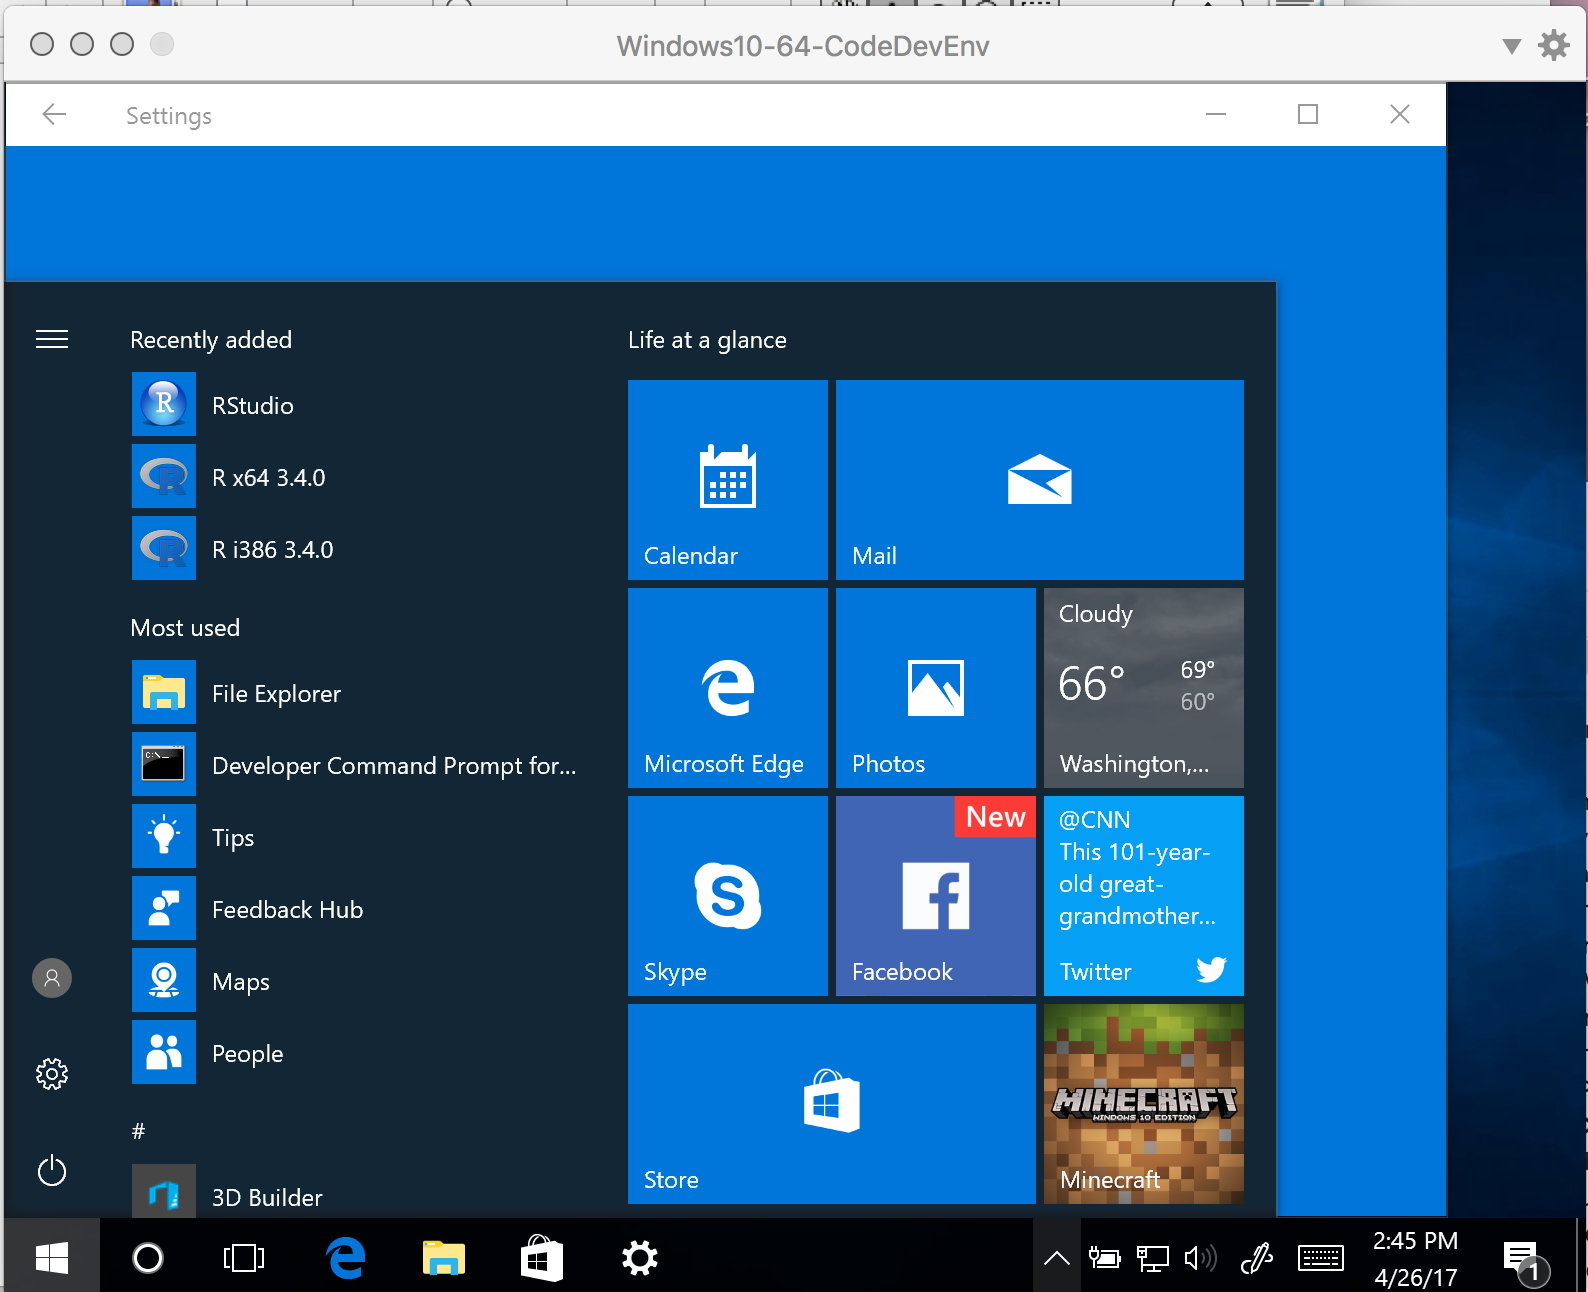
\includegraphics[width=4.5in]{./1-Introduction/verifyInstall.jpg} 
   \caption{Here we see the program is installed, now run \textbf{R Studio} to verify the install}
%   \label{fig:example}
\end{figure}

\begin{figure}[h!] %  figure placement: here, top, bottom, or page
   \centering
   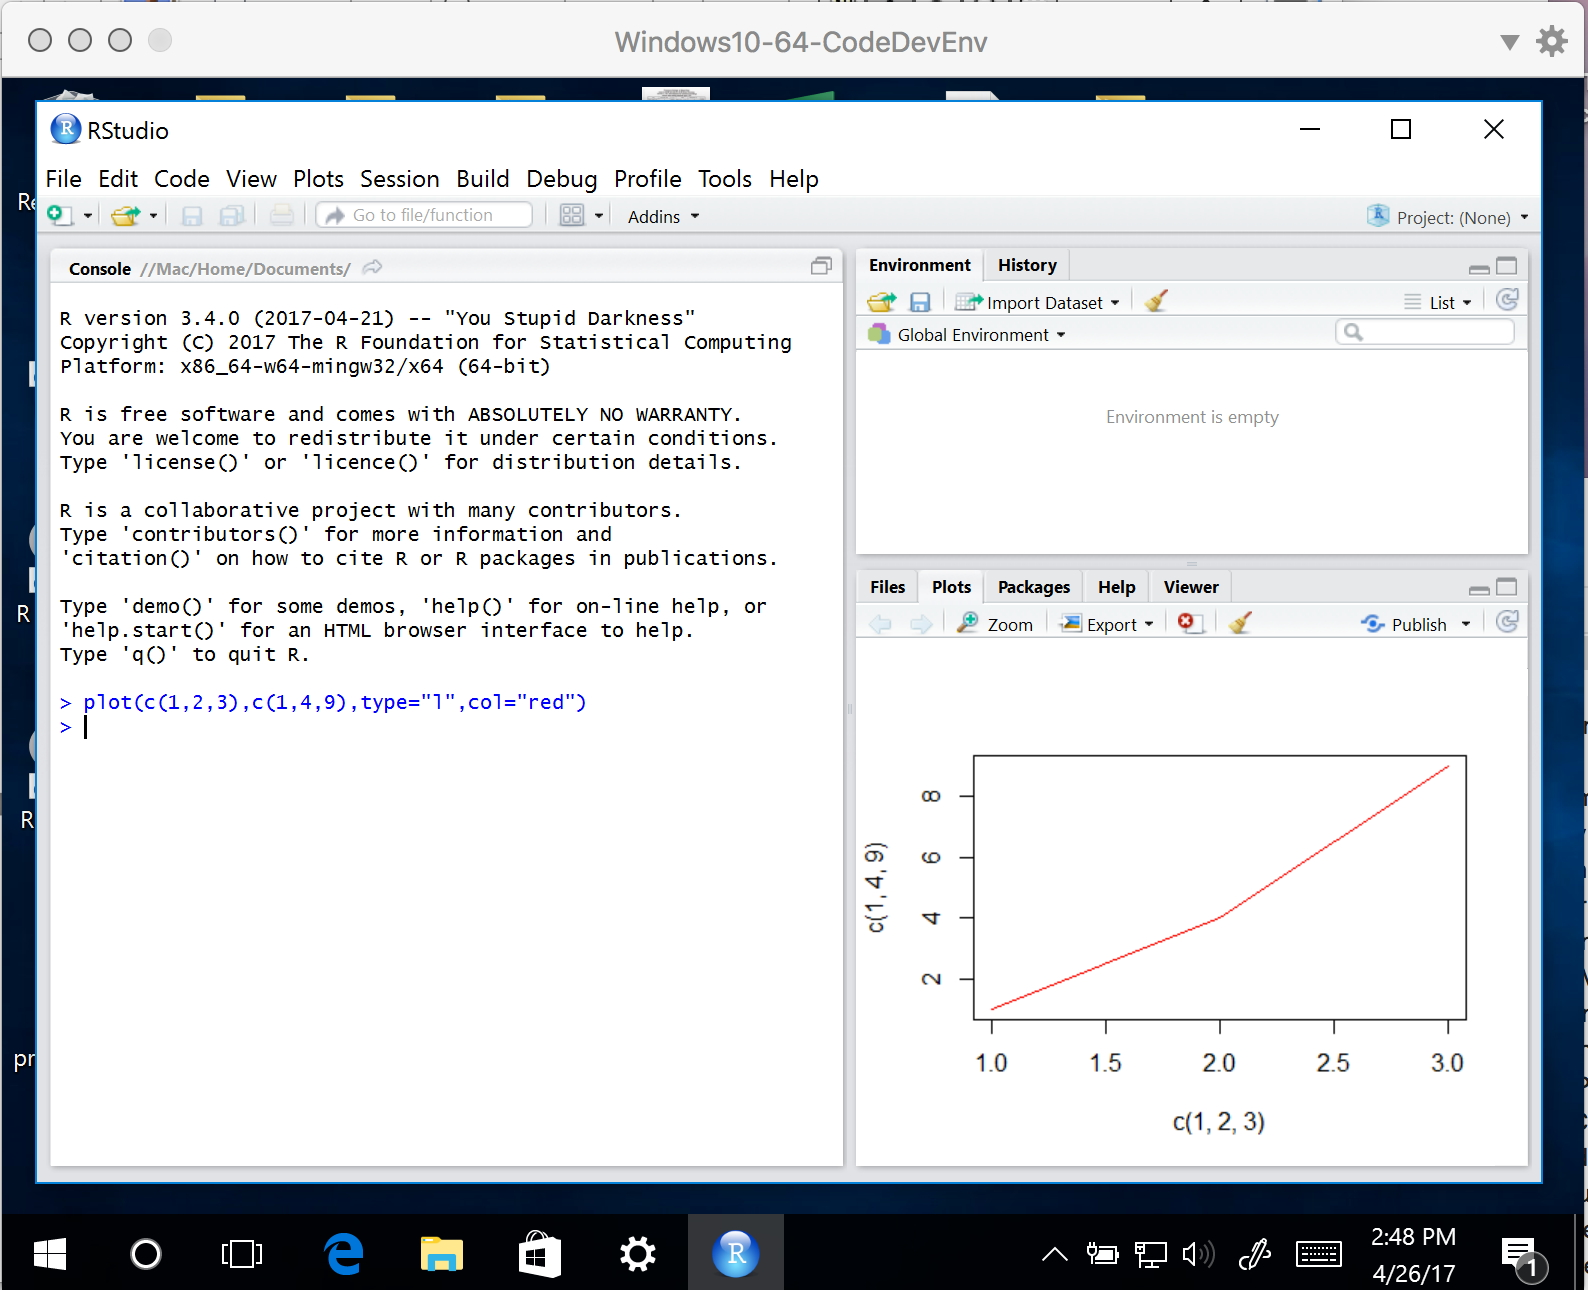
\includegraphics[width=4.5in]{./1-Introduction/verifyInstall2.jpg} 
   \caption{Type \texttt{plot(c(1,2,3),c(1,4,9),type="l",col="red")} into the console window.  A plot should be generated as shown}
%   \label{fig:example}
\end{figure}

\newpage~
\newpage~
\newpage~
\newpage~
\newpage~
\newpage~
\newpage~
Yipee!  It is running.  You can install additional packages now or later.  You should now have sufficient computation capability for the course.  
\clearpage

\subsubsection{Macintosh OSX Users}
[Replicate Windows using MacOS screen captures]
The purpose of this section is to demonstrate how to get \textbf{R} running on a Macintosh computer.\footnote{I assume no-one will be using a PPC-Based Mac.  If so, the CRAN does have PPC builds of R, but R Studio is not available; you would have to build from the source code.}  
This document assumes the following:
\begin{enumerate}
\item You have internet connection.
\item You have sufficient user privileges to install software on your machine.  (If it is your personal machine, the install may request your password, but should install.)
\item You have 60MB or so of vacant disk space on the system directory.
\end{enumerate}

The step-by-step guide is presented as a series of screen captures.  Obviously adjust inputs to fit your machine.  The version in these screen captures is quite dated --- use the most recent, stable version offered on CRAN (Comprehensive R Archive Network).\footnote{I have updated the screen captures for Windows 10 --- so these should replicate the steps.}

\begin{figure}[h!] %  figure placement: here, top, bottom, or page
   \centering
   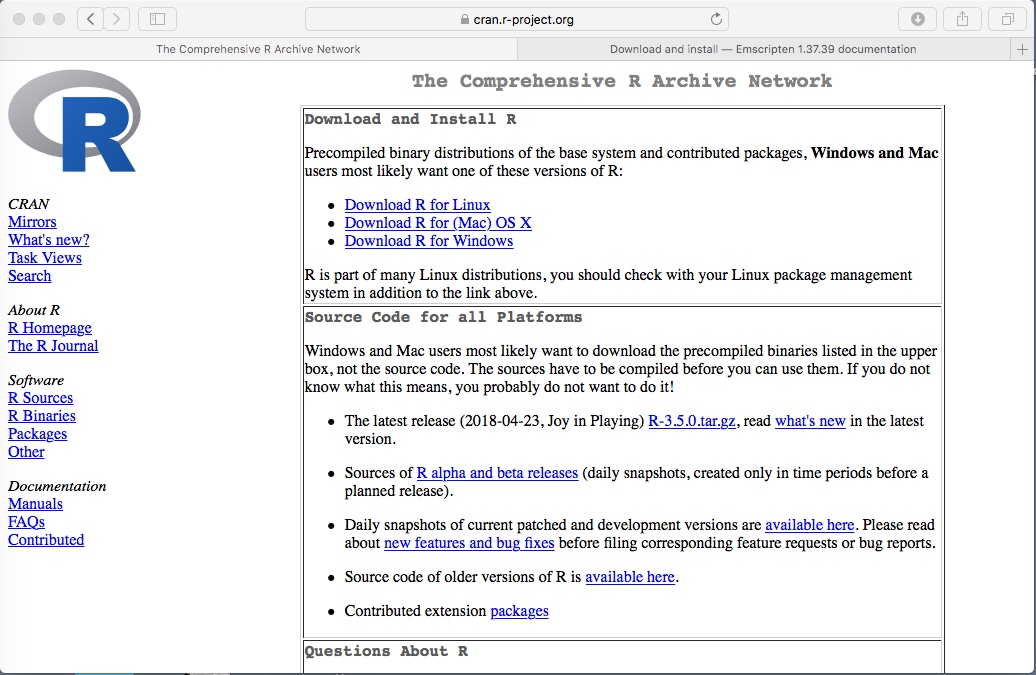
\includegraphics[width=5in]{./1-Introduction/GoogleRonMac.jpeg} 
   \caption{Google ``R'' (alternatively google CRAN)}
%   \label{fig:example}
\end{figure}

\begin{figure}[h!] %  figure placement: here, top, bottom, or page
   \centering
   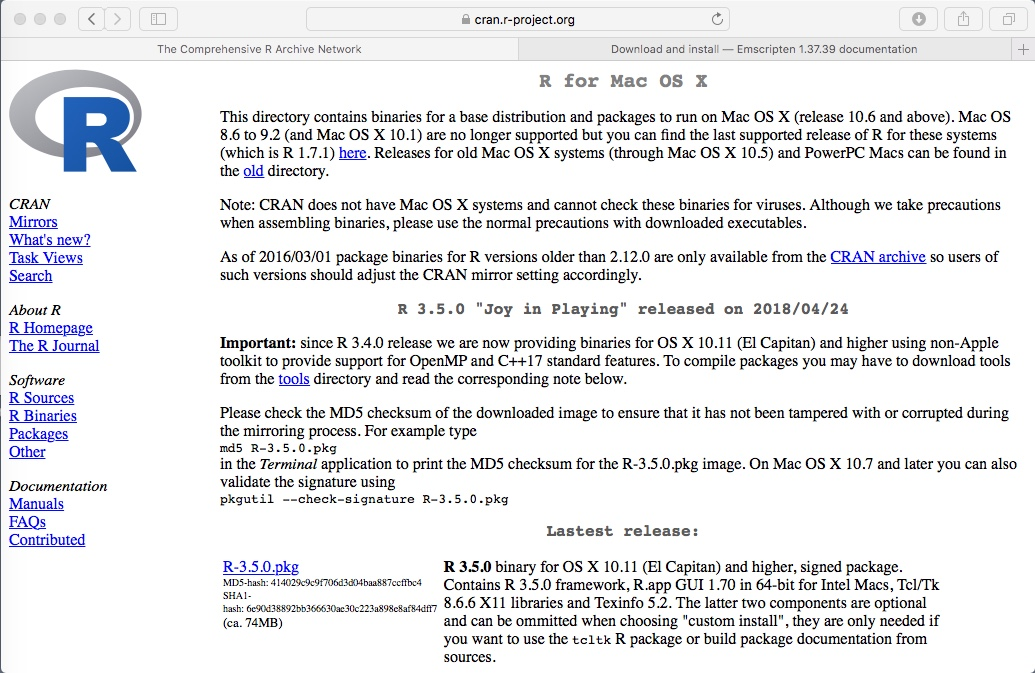
\includegraphics[width=5in]{./1-Introduction/SelectOS-Mac.jpeg} 
   \caption{Select MacOS operating system link}
%   \label{fig:example}
\end{figure}

\begin{figure}[h!] %  figure placement: here, top, bottom, or page
   \centering
   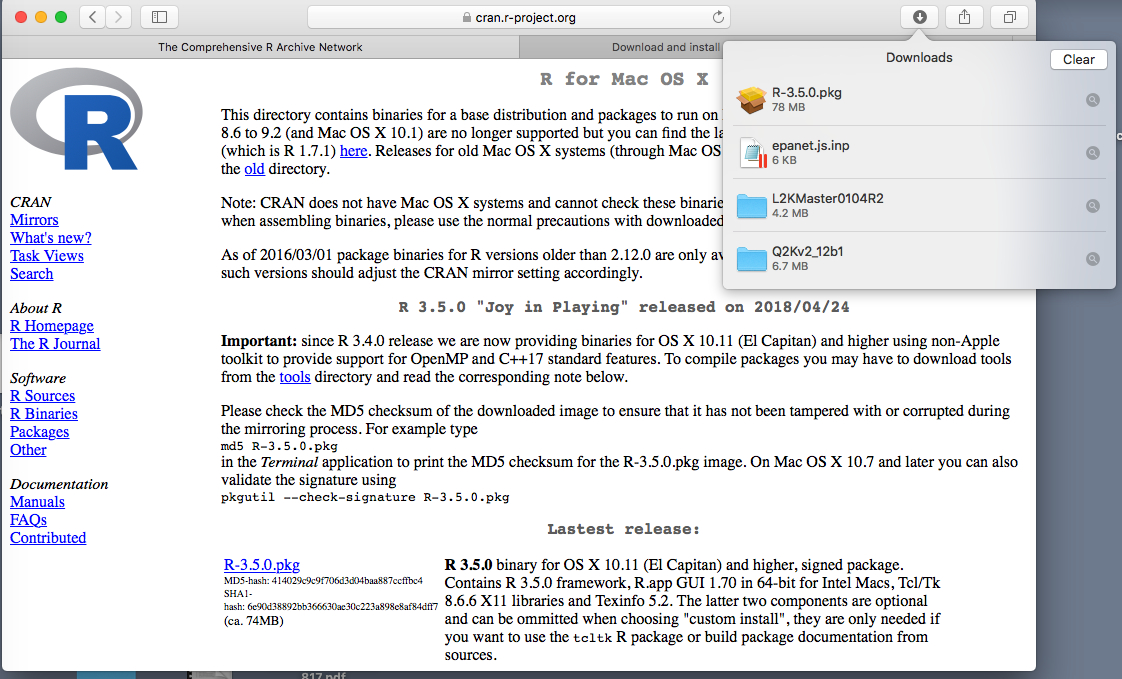
\includegraphics[width=5in]{./1-Introduction/DownloadR-pkg.jpg} 
   \caption{Download the R Installer}
%   \label{fig:example}
\end{figure}

\begin{figure}[h!] %  figure placement: here, top, bottom, or page
   \centering
   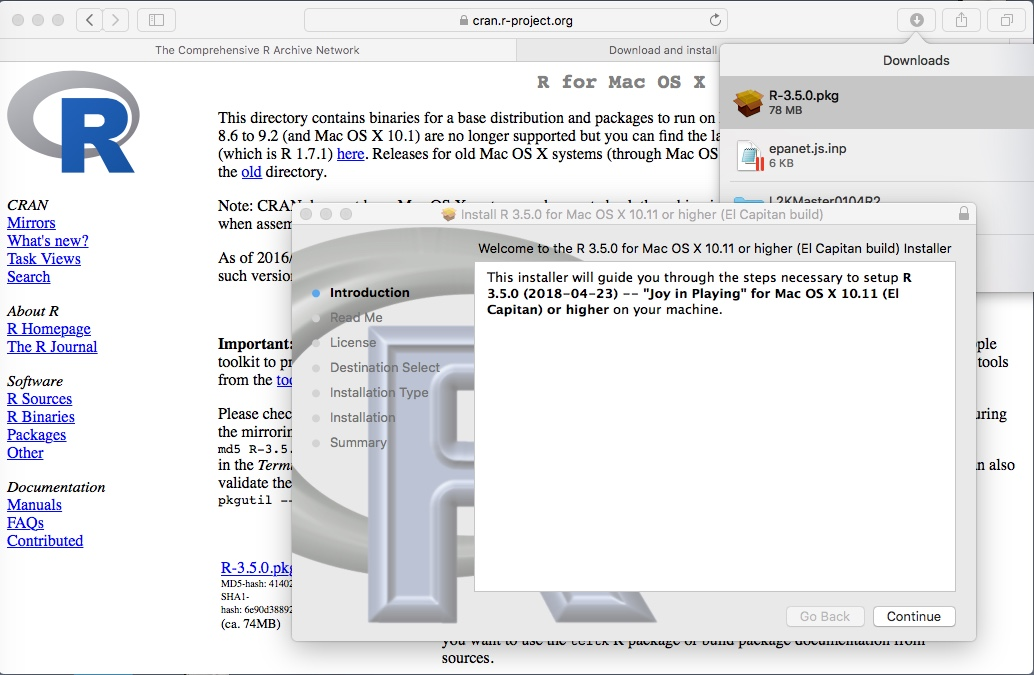
\includegraphics[width=5in]{./1-Introduction/RunInstallerMAC.jpeg} 
   \caption{Run the installer, accept the defaults}
%   \label{fig:example}
\end{figure}

\begin{figure}[h!] %  figure placement: here, top, bottom, or page
   \centering
   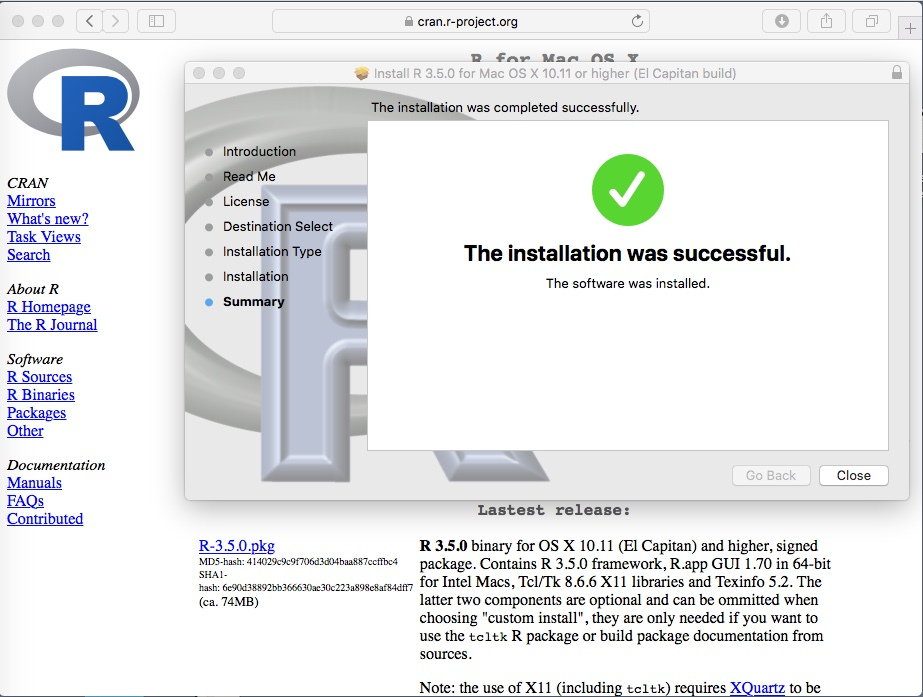
\includegraphics[width=5in]{./1-Introduction/MacSuccessR.jpeg} 
   \caption{Successful install}
%   \label{fig:example}
\end{figure}

\begin{figure}[h!] %  figure placement: here, top, bottom, or page
   \centering
   
\includegraphics[width=5in]{./1-Introduction/GoogleRStudio4Mac.jpeg} 
   \caption{Google R Studio}
%   \label{fig:example}
\end{figure}

\begin{figure}[h!] %  figure placement: here, top, bottom, or page
   \centering
   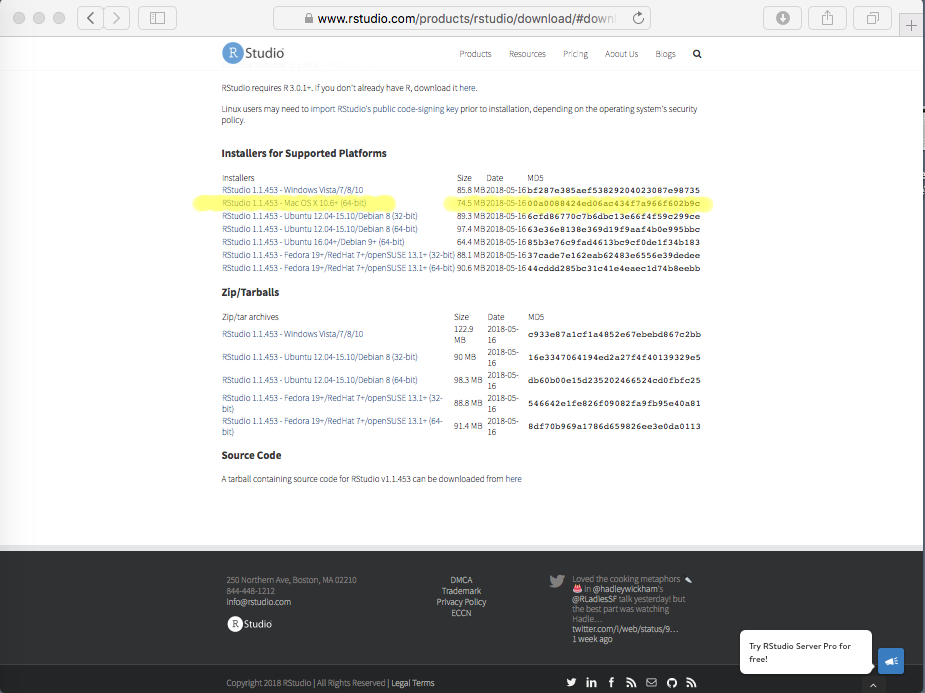
\includegraphics[width=5in]{./1-Introduction/SelectRStudioInstaller.jpg} 
   \caption{Select R Studio installer (for MacOS)}
%   \label{fig:example}
\end{figure}

\begin{figure}[h!] %  figure placement: here, top, bottom, or page
   \centering
   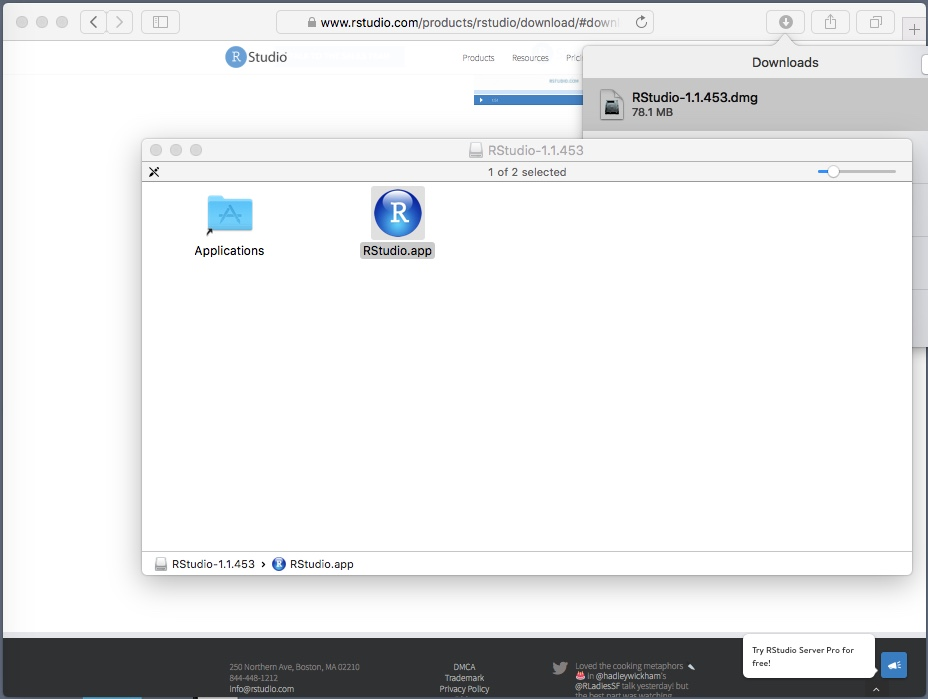
\includegraphics[width=5in]{./1-Introduction/MountDiskImage.jpeg} 
   \caption{Mount the disk image.  Then drag the R Studio icon on top of the Applications link -- this action will install the program}
%   \label{fig:example}
\end{figure}

\begin{figure}[h!] %  figure placement: here, top, bottom, or page
   \centering
   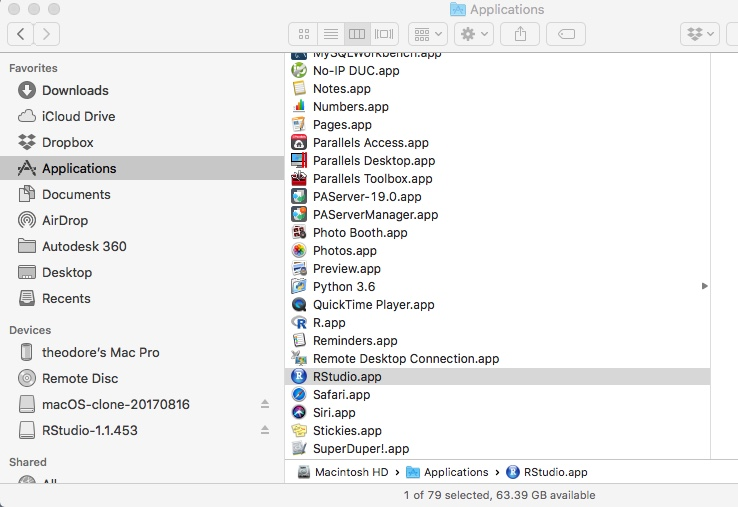
\includegraphics[width=5in]{./1-Introduction/LaunchRStudioMac.jpeg} 
   \caption{Start R Studio (in Applications directory, double click on the icon)}
%   \label{fig:example}
\end{figure}

\begin{figure}[h!] %  figure placement: here, top, bottom, or page
   \centering
   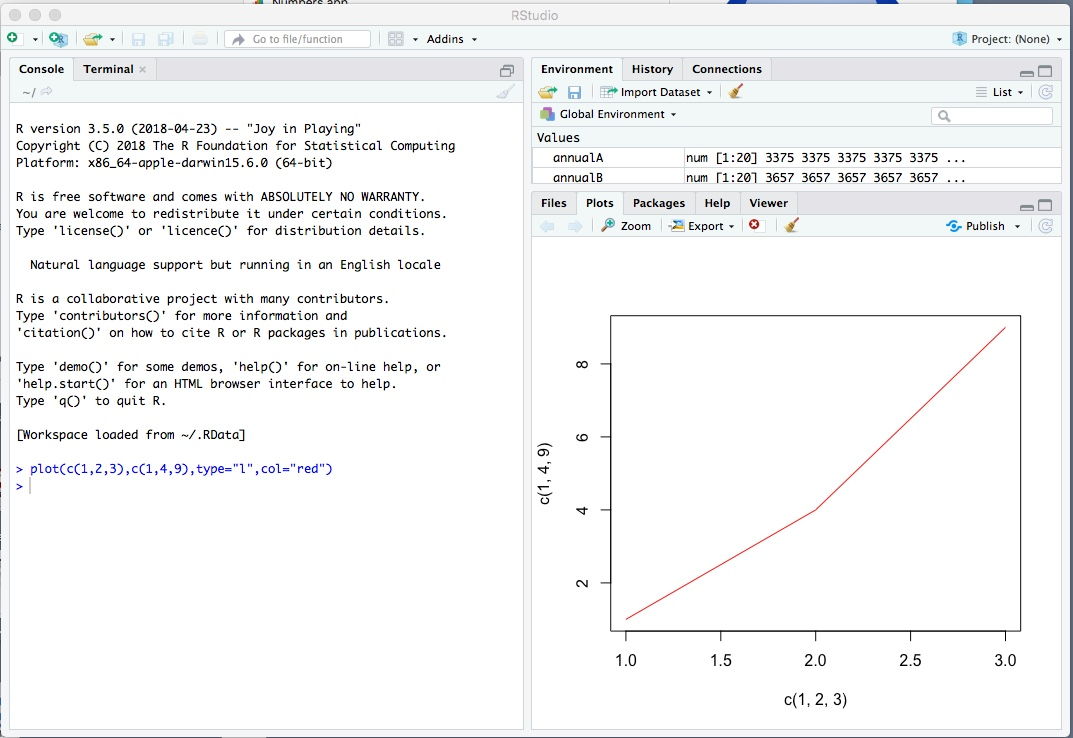
\includegraphics[width=5in]{./1-Introduction/TestMacInstall.jpeg} 
   \caption{Type in some R script and viola -- it produces a simple plot}
%   \label{fig:example}
\end{figure}

\newpage~
\newpage~
\newpage~
\newpage~
\newpage~
Yipee!  It is running.  You can install additional packages now or later.  You should now have sufficient computation capability for the course.  



\clearpage
\subsubsection{Linux Users}
The purpose of this section is to demonstrate how to get \textbf{R} and \textbf{R Studio}  running on a Linux computer.  
This document assumes the following:
\begin{enumerate}
\item You have internet connection.
\item You have sufficient user privileges to install software on your machine.  
Generally, if it is your own machine then you have superuser (root) privileges.
If it is some network machine maintained by someone else you probably don't have such priviliges.
The examples here use the \texttt{sudo <command>} to do the installs -- on my machine the password I enter is my user password (and not the root password).  
Alternativley you can switch user \texttt{su} to root, and run the installs as root -- this approach is considerably more dangerous in terms of wrecking your operating system that using the \texttt{sudo} approach.
\item You have 60MB or so of vacant disk space on the system directory.
\end{enumerate}

The step-by-step guide is presented as a series of screen captures.  Obviously adjust inputs to fit your machine.  
Use the most recent, stable version offered on CRAN (Comprehensive R Archive Network).

\begin{figure}[h!] %  figure placement: here, top, bottom, or page
   \centering
   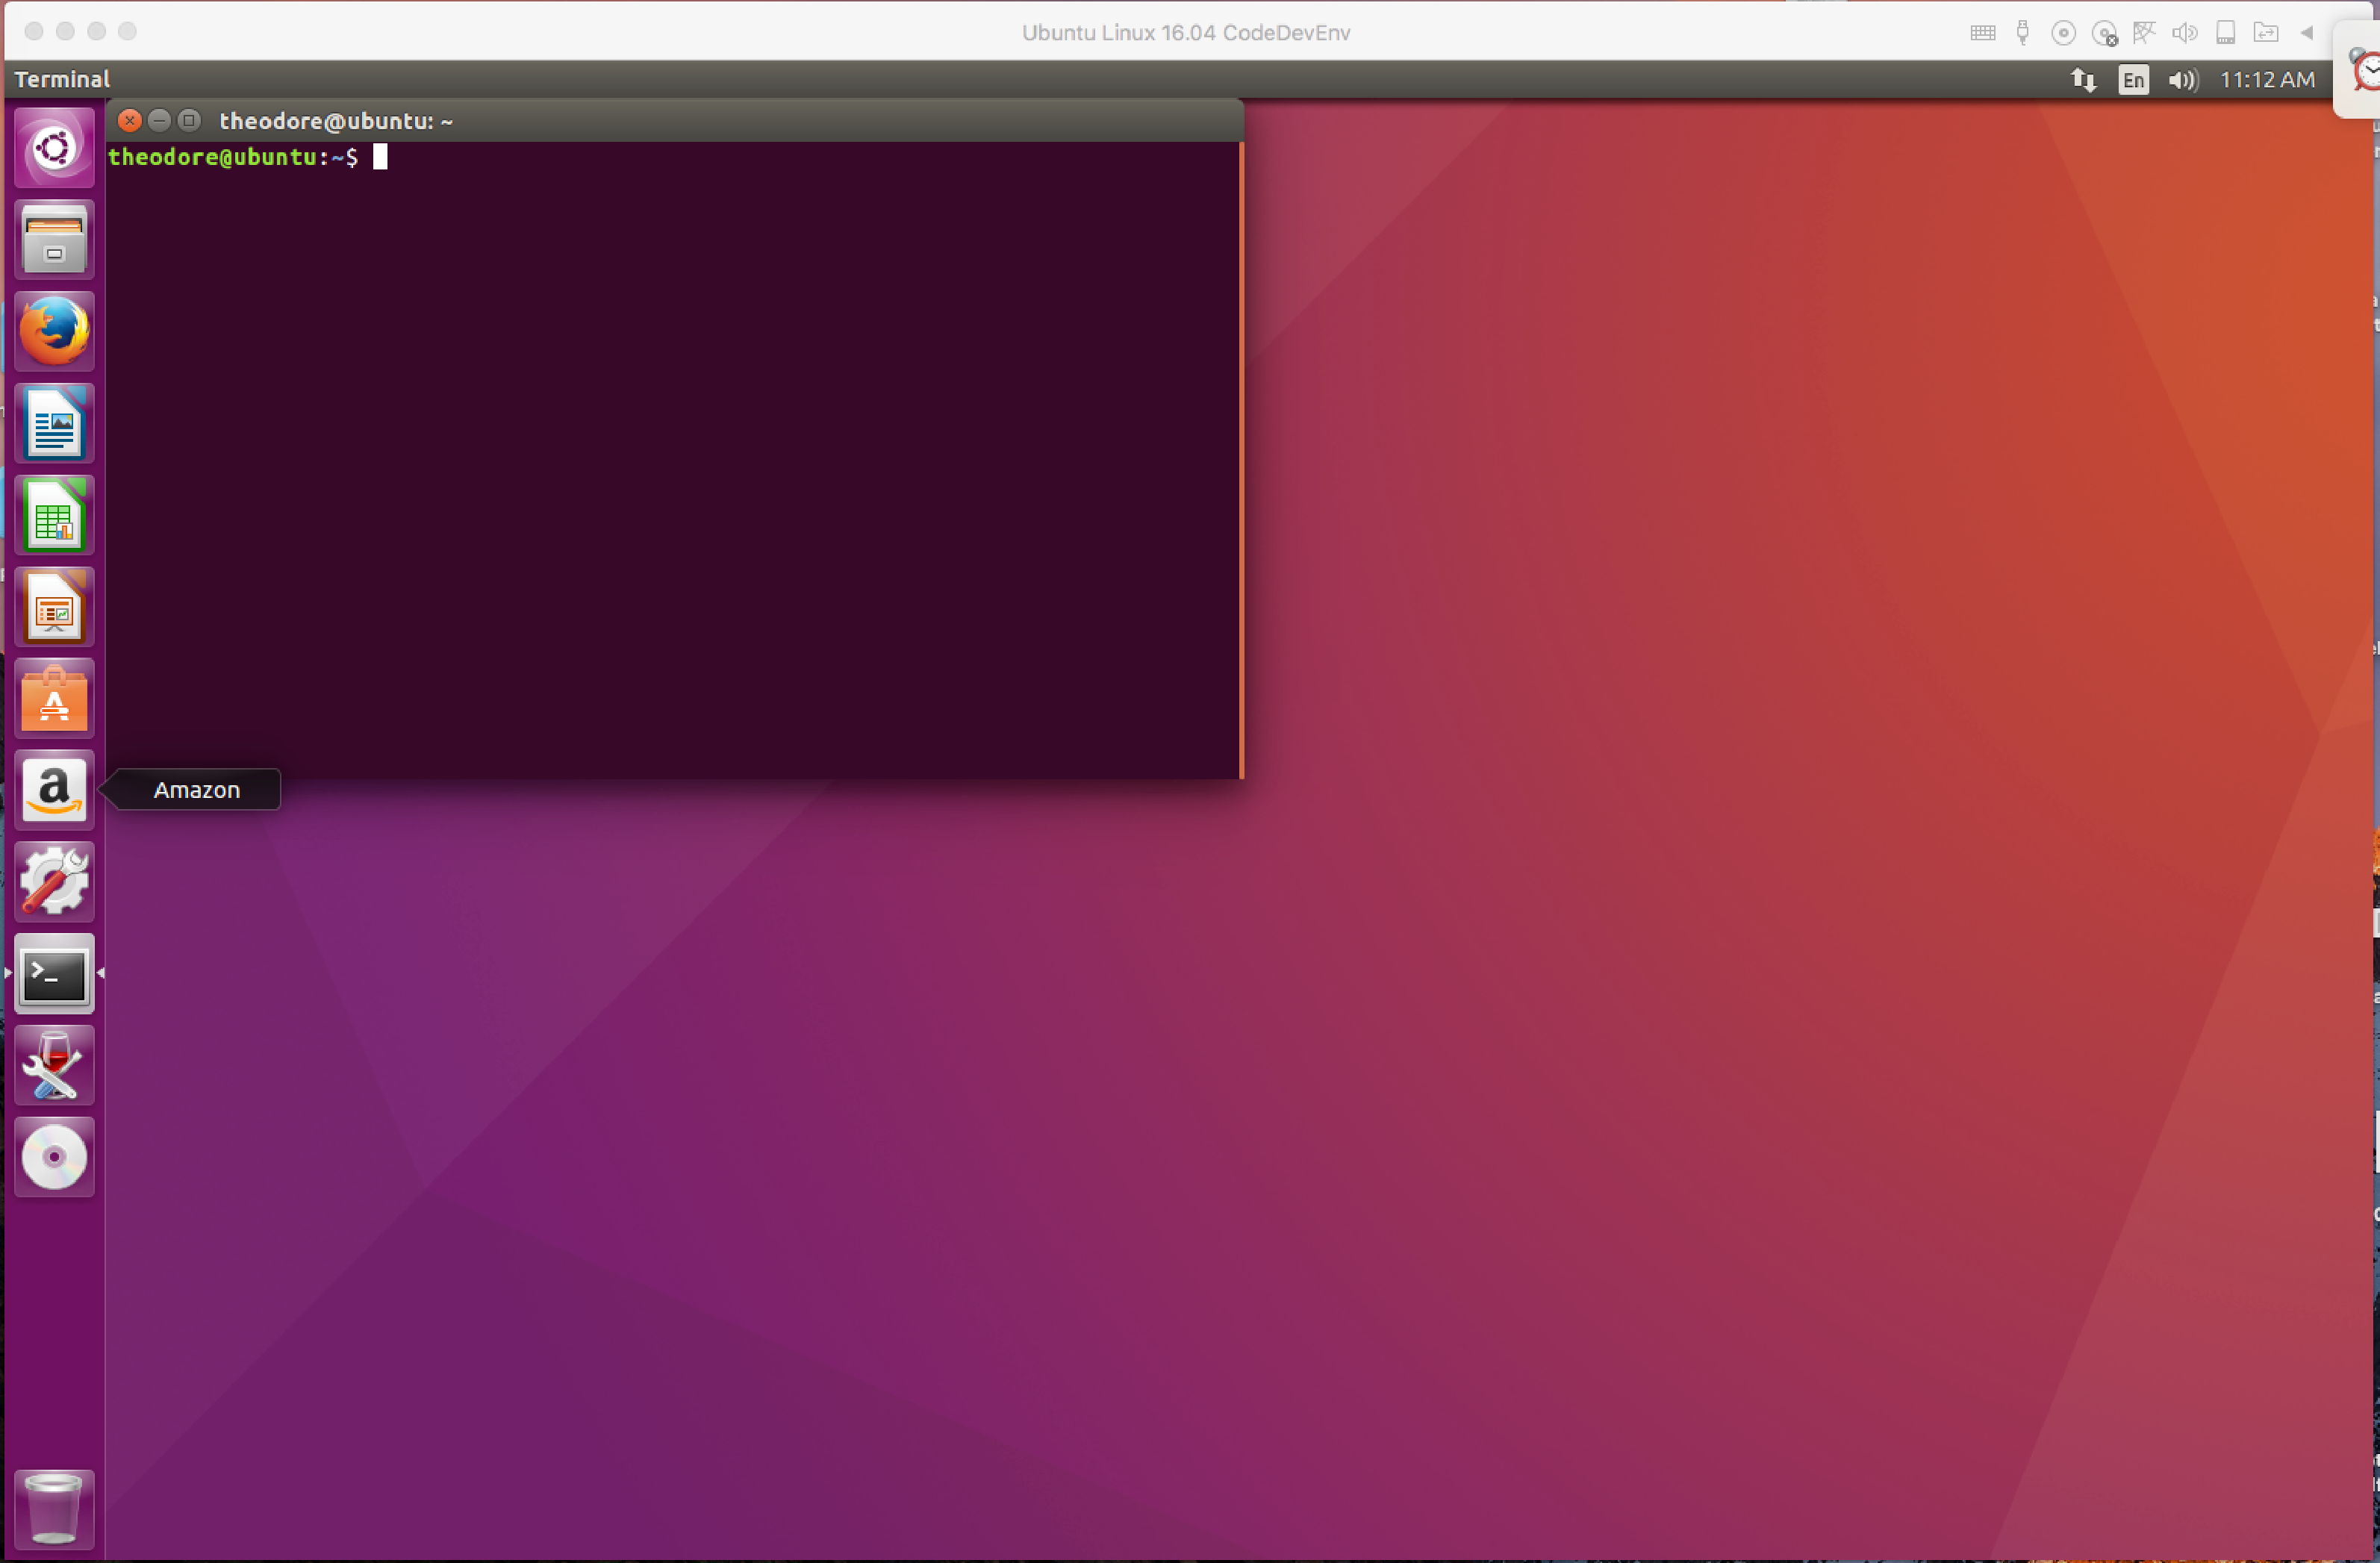
\includegraphics[width=5in]{./1-Introduction/LinuxTerminalPrompt.pdf} 
   \caption{Terminal Prompt in Linux}
%   \label{fig:example}
\end{figure}

To get started we need to install \textbf{R}.  
The easiest method is to use the package manager -- my Linux distribution is Ubuntu 16.XX.  
It is built from the debian distribution and uses the \texttt{apt} package manager.
The package manager is pretty cool because when we request a package it finds the package and its dependencies, downloads everything needed and then we can install.
In earlier times (the 1990's) using the Red Hat Package Manager (\texttt{rpm}) one would have to find the dependencies themselves (in all fairness \texttt{rpm} would identify the dependencies and suggest where to find them!).  So here we go, first open a terminal in Linux.

Next in the terminal window issue the command \texttt{sudo apt install r-cran-littler}.

\begin{figure}[h!] %  figure placement: here, top, bottom, or page
   \centering
   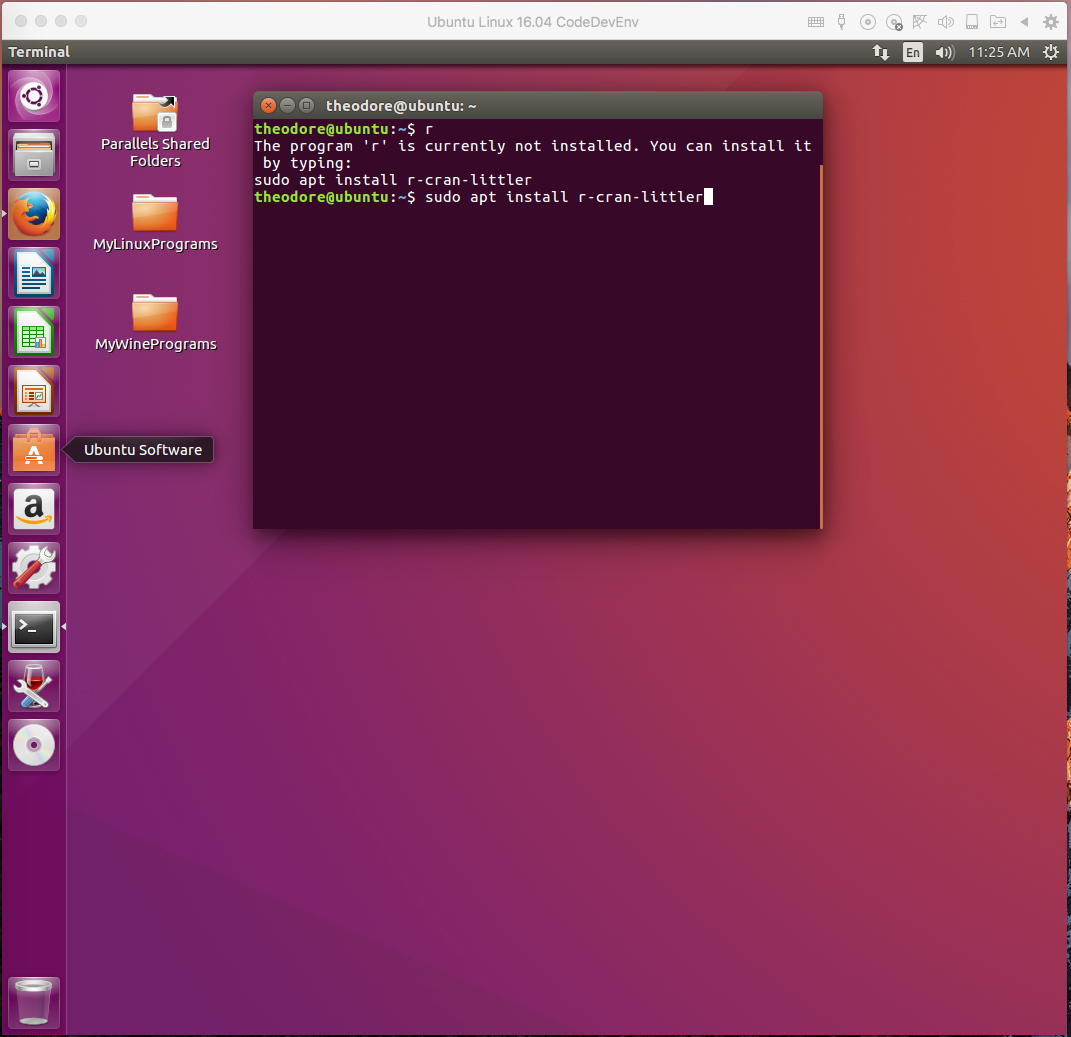
\includegraphics[width=4.5in]{./1-Introduction/LinuxInstallR.jpg} 
   \caption{Install R using the \texttt{apt} package manager (or \texttt{rpm} if using a red hat variant)}
%   \label{fig:example}
\end{figure}

When you press return, the computer should ask for a password -- use your user password; if you have install privileges this will work.  
If not, you will have to switch user to root and either add your user account to the group \texttt{wheel}, return to your account -- or just install as root.

Next the install will begin and may take a few minutes.  
Usually there is a lot of installer messages that run across the screen (kind of like in ``The Matrix'').
The \texttt{apt} utility is downloading files and binging them to resources on the system so that \textbf{R} can run.
Eventually it should get to the end of the install and may look something like the next screen capture.

Our next task is to verify that the install was successful.
Usually failure is obvious, but not always.
I find the easiest way to verify that the operating system thinks the software is installed is issue the command to run the program with the version switch active.
In this case, issue the command \texttt{r --version}.
This command will try to run \textbf{R}, and will return the version number (or build number). 

In the next screen capture when we run the command we see that the version number is \textbf{R} version 3.2.2.
The version numbering system is typical for all software -- it identifies something like this is the second subversion, of the second revision, of the third stable release. 

\begin{figure}[h!] %  figure placement: here, top, bottom, or page
   \centering
   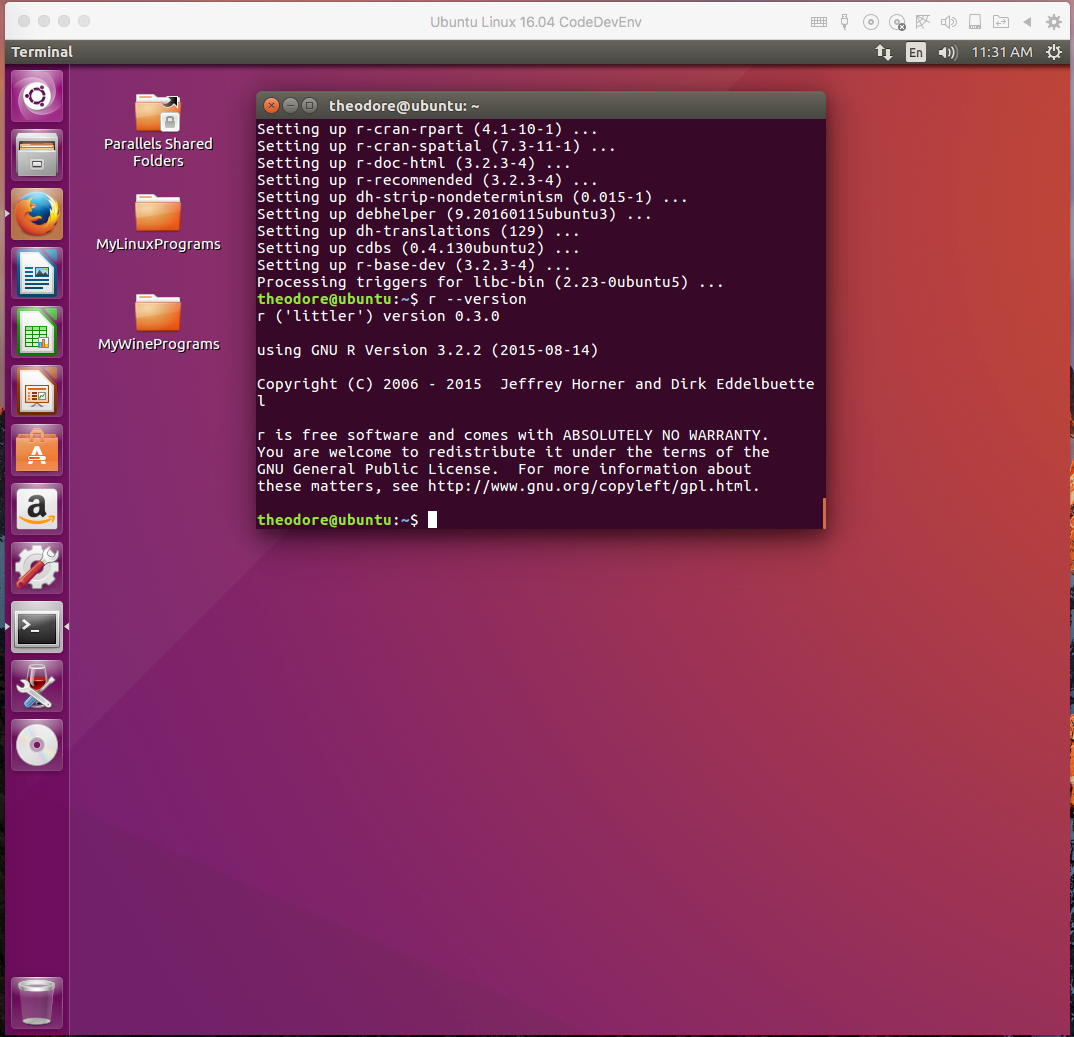
\includegraphics[width=5in]{./1-Introduction/LinuxRVersion.jpg} 
   \caption{Verify install of \textbf{R} using \texttt{r --version}}
%   \label{fig:example}
\end{figure}

The next step I recommend is to go ahead and download a development environment.
\textbf{R Studio} is an integrated development environment for \textbf{R}.   
We don't ``need'' it, but it enforces some discipline, gives us a place to store and modify \textbf{R}-scripts (little programs), and lets us see all of our work going on in one location.

To get \textbf{R Studio} we have to download it from the manufacturer, the copy we will use is free.  
Instead of \texttt{apt} this time I used Firefox to navigate to the \textbf{R Studio} website, then select download.

Next select the appropriate installer for your platform.
Be sure you are selecting an installer and not the source codes for the program.\footnote{In theory we could build the program from source using the make utility and (hopefully) already installed compilers -- this is for people with time, training, inclination and need.  We are going to use the already built binaries!}

We will download the 64-bit version (unless you have a 32-bit machine, then you need 32-bit software).
We need to select our Linux platform -- mine is Unbuntu/Debian.   
I also have a Red Hat/SuSe machine, so if I were using that machine, i would select its software.

\begin{figure}[h!] %  figure placement: here, top, bottom, or page
   \centering
   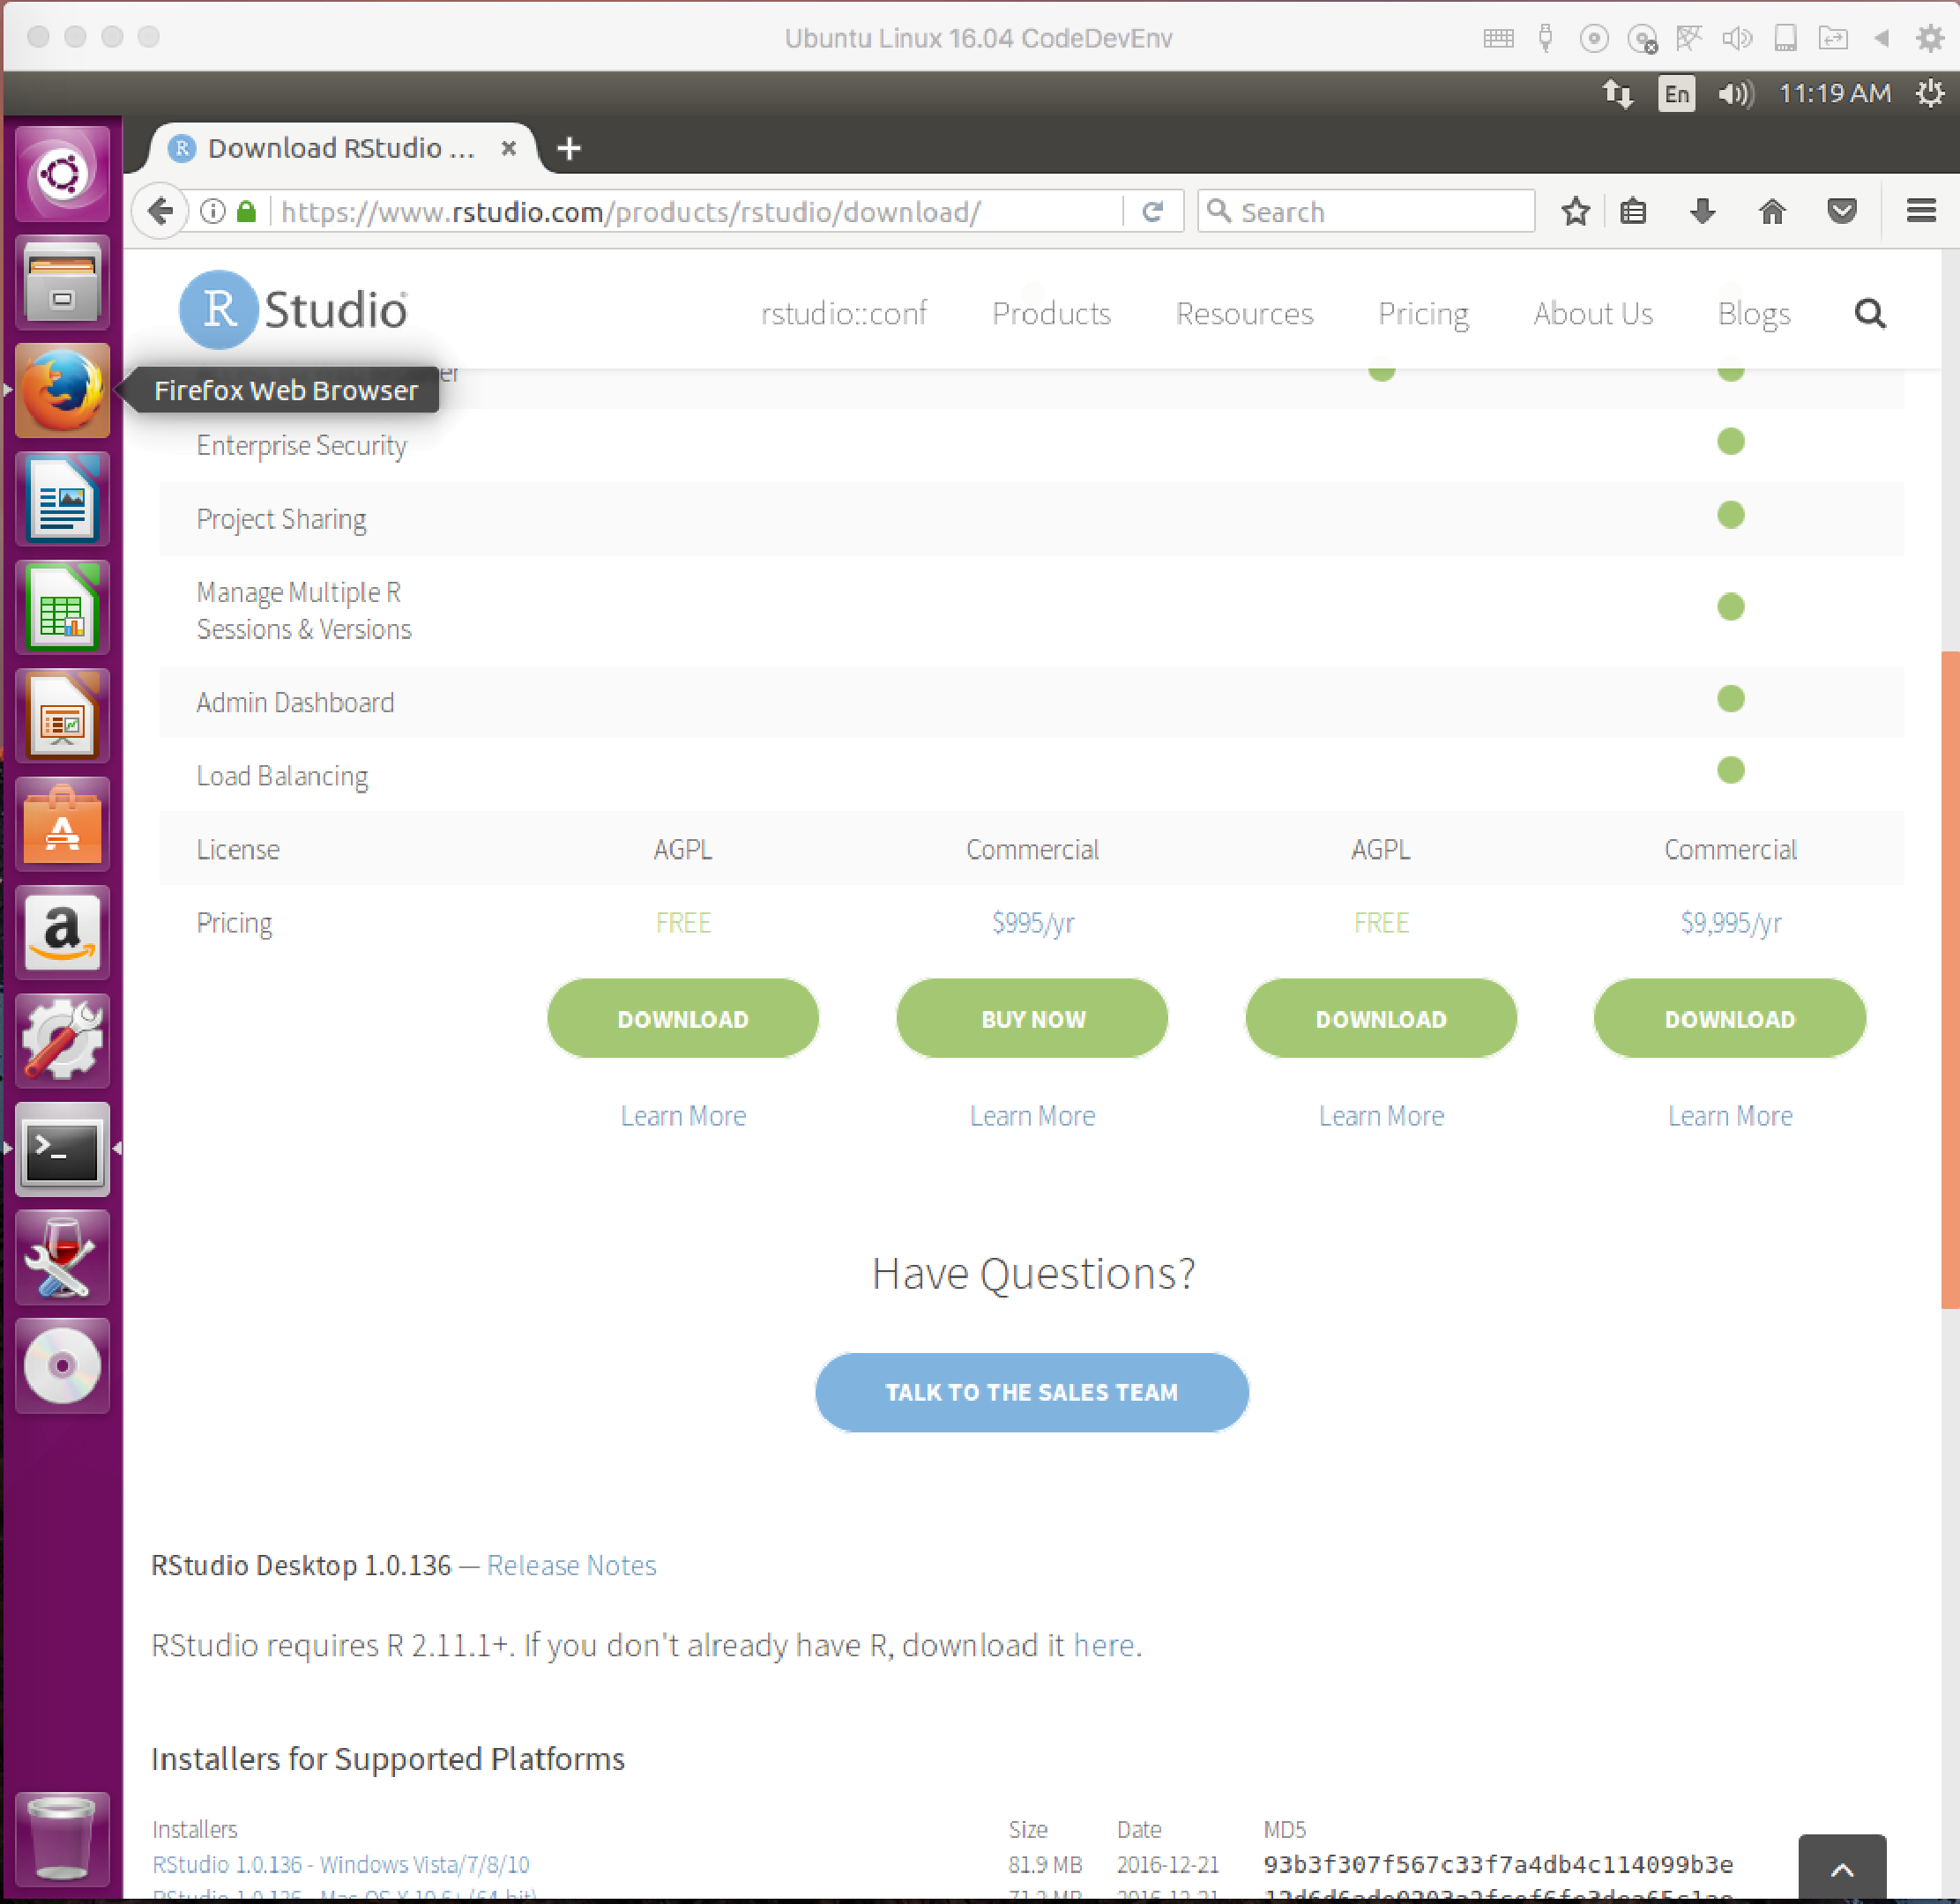
\includegraphics[width=3.5in]{./1-Introduction/LinuxRStudio.pdf} 
   \caption{Browser search for \textbf{R Studio}; go to downloads.  We are going to select the free (leftmost) column}
%   \label{fig:example}
\end{figure}

\begin{figure}[h!] %  figure placement: here, top, bottom, or page
   \centering
   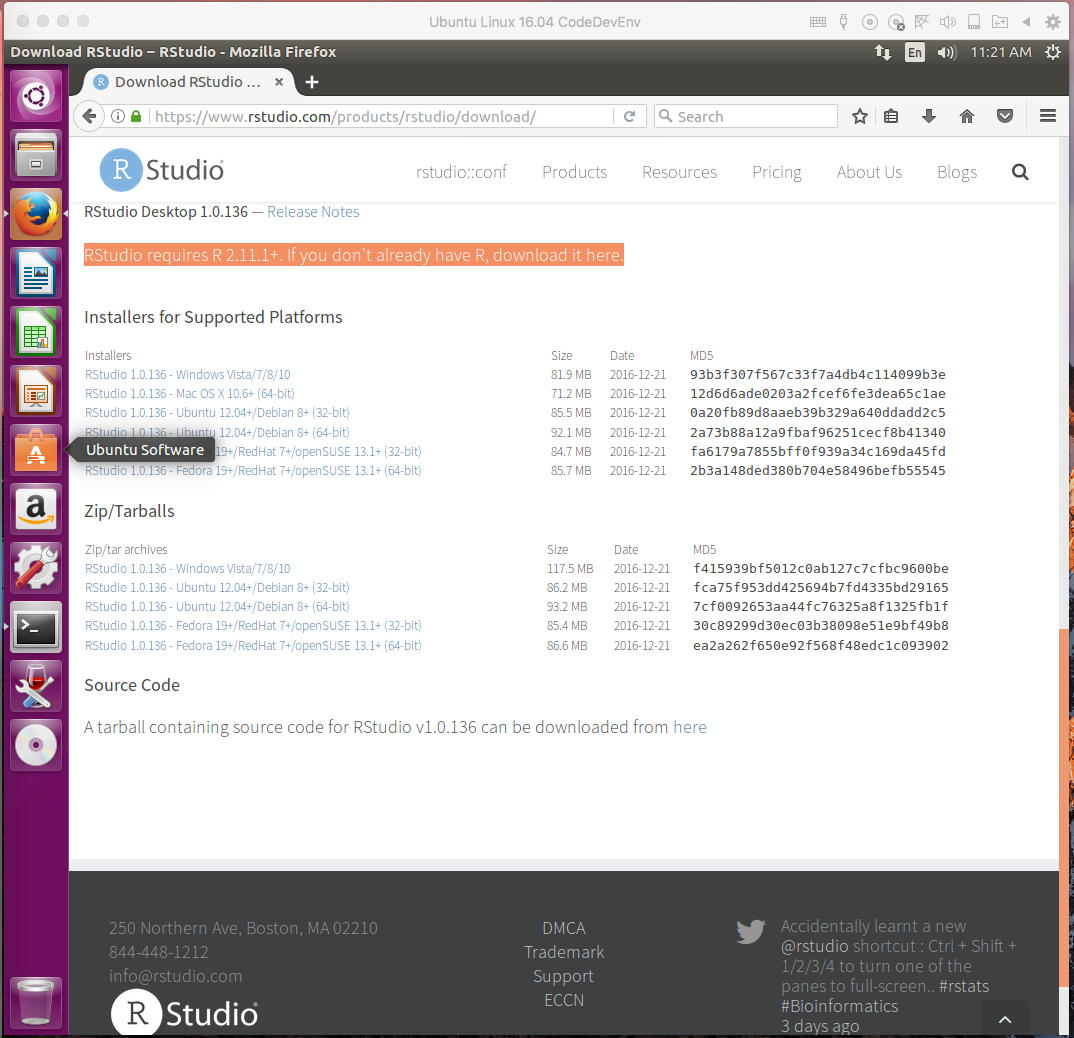
\includegraphics[width=3.5in]{./1-Introduction/LinuxRStudioDownload.jpg} 
   \caption{Download the version of \textbf{R Studio}; in this case 64-bit for Ubuntu Linux (what I am using).  
   My computer asks if upon download if I want to run the installer, of course select YES}
   \label{fig:LinuxRStudioDownload}
\end{figure}

\clearpage

Figure \ref{fig:LinuxRStudioDownload} is the selection page for selecting the installers.  
Once I select the package the computer starts the download, and asks me if I want to run the installer, as in Figure \ref{fig:LinuxRStudioInstall}



\begin{figure}[h!] %  figure placement: here, top, bottom, or page
   \centering
   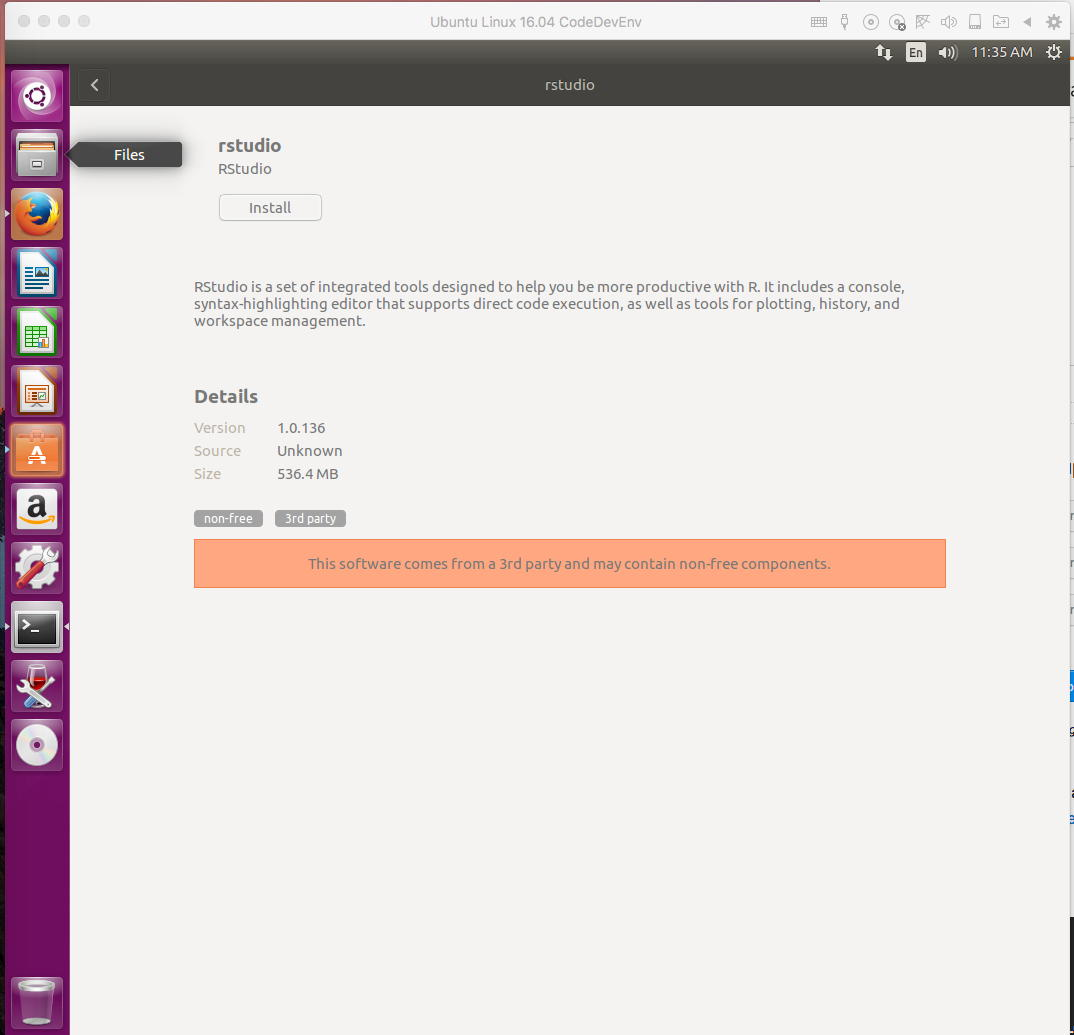
\includegraphics[width=3.5in]{./1-Introduction/LinuxRStudioInstall.jpg} 
   \caption{Here we select install, and let the installer do its thing}
   \label{fig:LinuxRStudioInstall}
\end{figure}

Selecting yes, the installer will attempt to install \textbf{R Studio} onto my computer. 
Once installation is complete, the program is ready for a validation (of install) run.

\begin{figure}[h!] %  figure placement: here, top, bottom, or page
   \centering
   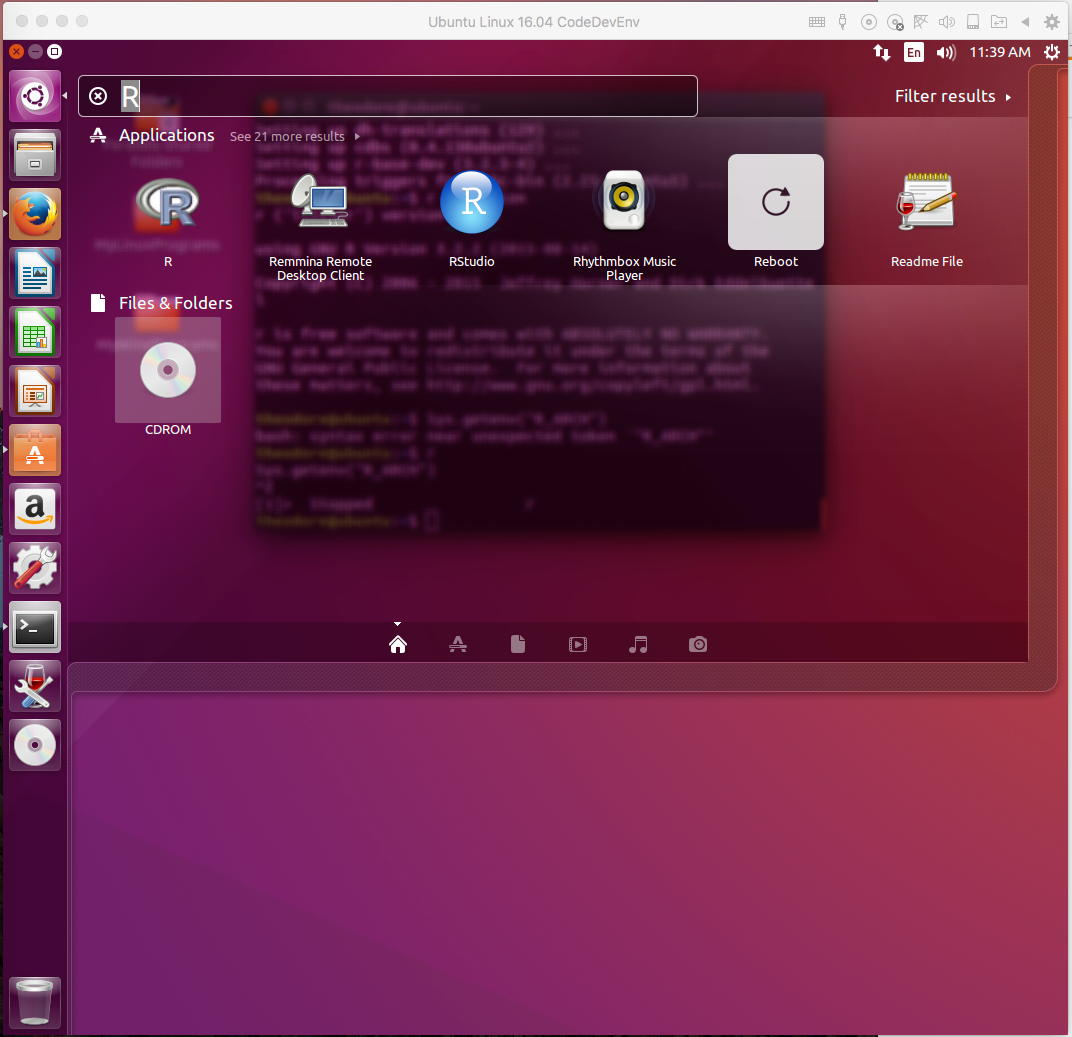
\includegraphics[width=3.35in]{./1-Introduction/LinuxRStudioSelect.jpg} 
   \caption{To launch \textbf{R Studio}, either select in the applications folder (or type in the terminal \texttt{rstudio}}
\label{fig:LinuxRStudioSelect}
\end{figure}

\clearpage
Figure \ref{fig:LinuxRStudioSelect} is a screen capture after installation using the Unbuntu program manager window.  
Both \textbf{R} and \textbf{R Studio} are available.  

Either select \textbf{R Studio} to launch it, or type in a terminal window \texttt{rstudio} and the IDE should launch.
The IDE itself is a bit complicated, but actually enables us to keep better track of our work and ultimately saves time.
MatLab users should notice that the interface looks quite similar (at least it does to me) -- its also the same concept.

Figure \ref{fig:LinuxRStudioOpen} is the result of launching the program.  
The left side of the IDE is an \textbf{R} console -- exactly what would occur if we had just started \textbf{R}.
The right side of the IDE is divided into an upper and lower panel.  
Each panel  provides information about our programming environment at any instant -- and the content is selectable from the icons at the top of each panel.


\begin{figure}[h!] %  figure placement: here, top, bottom, or page
   \centering
   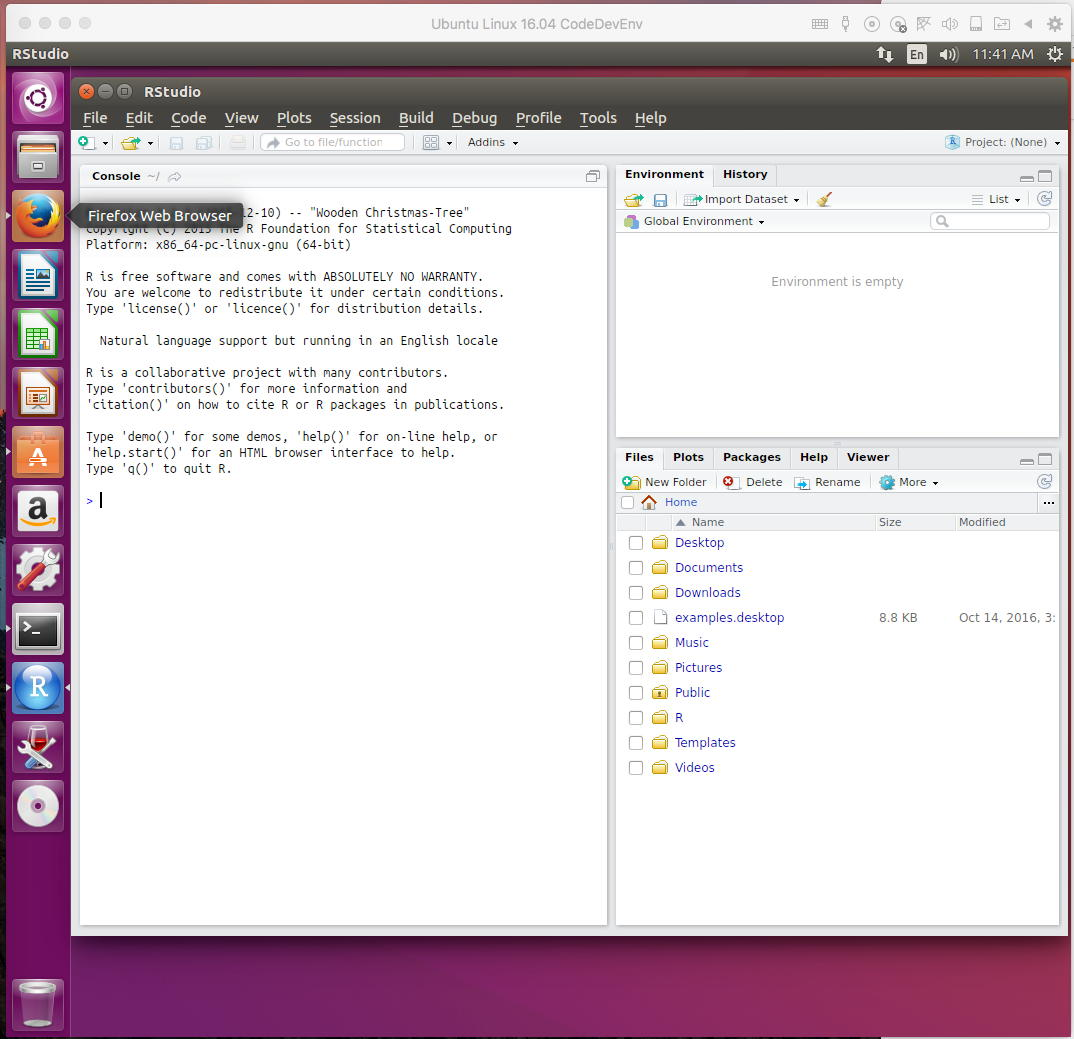
\includegraphics[width=4.5in]{./1-Introduction/LinuxRStudioOpen.jpg} 
   \caption{Upon opening you should have the following integrated development environment (IDE).   The left panel is exactly what you would obtain if
   you just type \texttt{r} in the terminal window.  }
   \label{fig:LinuxRStudioOpen}
\end{figure}

The next few figures are a step-by-step example to introduce \textbf{R Studio} as well as test if it installed correctly.
We could simply type in the \textbf{R} console within the IDE, but instead to get into the habit of saving our work, we will open a new scripting file.
\clearpage

Figure \ref{fig:LinuxRStudioNewFile} shows the process of selecting FILE/OPEN to create a new file to store our scripts.
We will type a few commands into the file and then run them.

\begin{figure}[h!] %  figure placement: here, top, bottom, or page
   \centering
   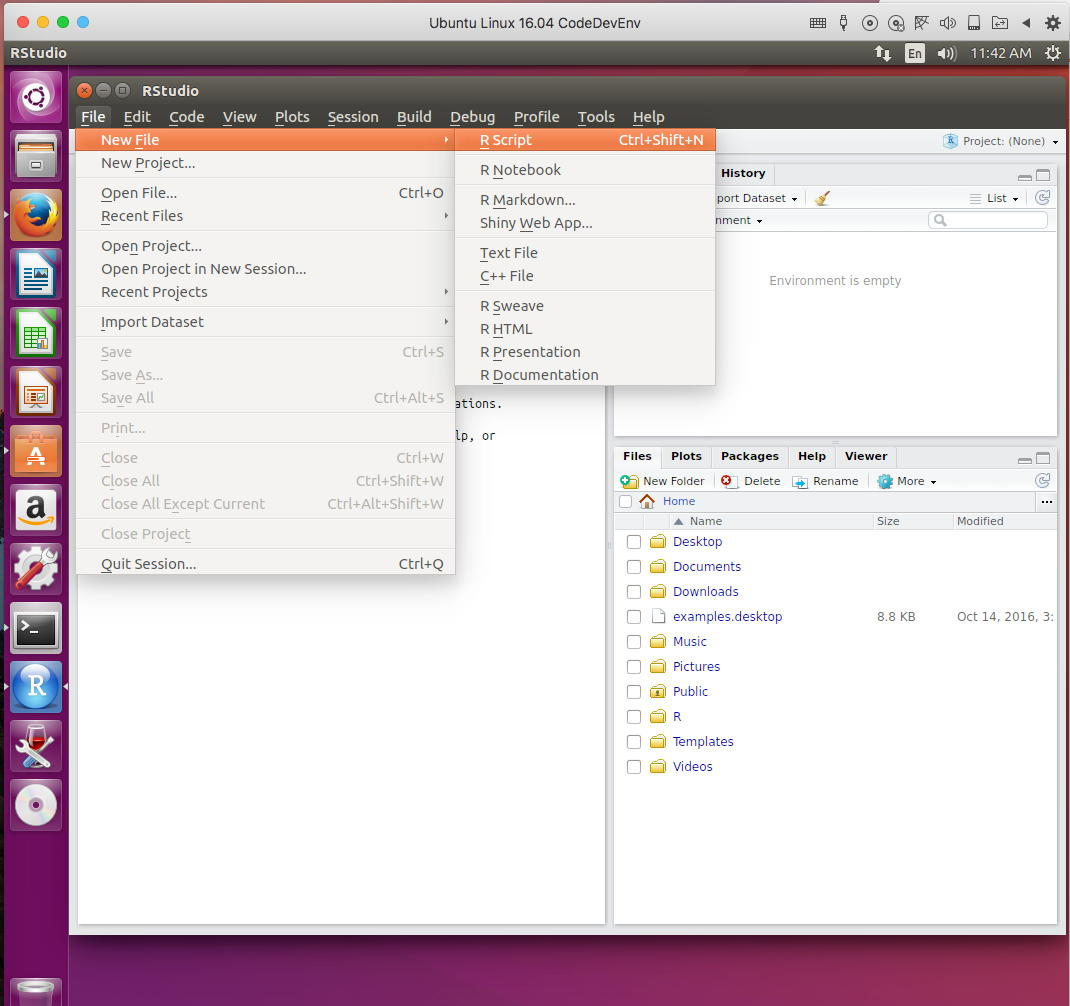
\includegraphics[width=4in]{./1-Introduction/LinuxRStudioNewFile.jpg} 
   \caption{Open a new file -- in this case as an \textbf{R-Script}}
   \label{fig:LinuxRStudioNewFile}
\end{figure}

\begin{figure}[h!] %  figure placement: here, top, bottom, or page
   \centering
   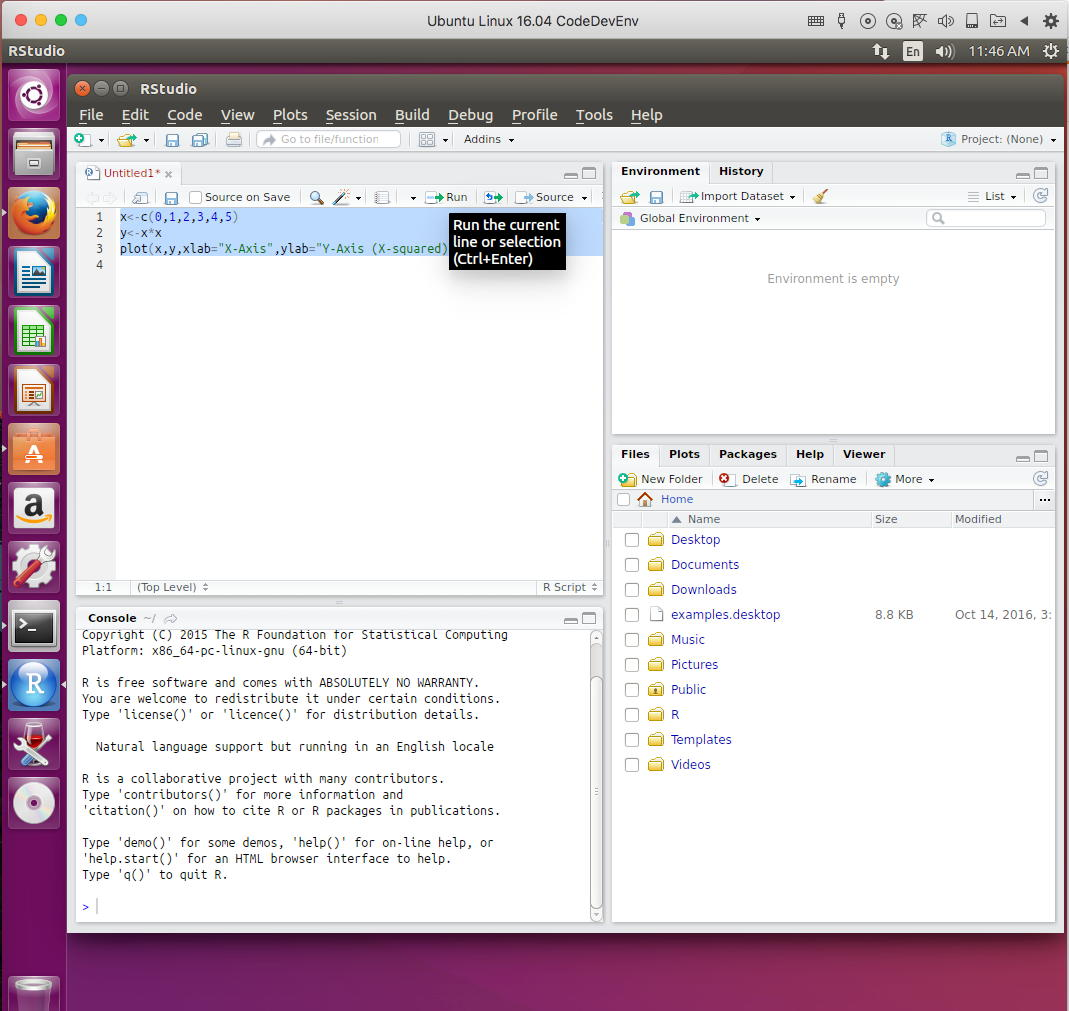
\includegraphics[width=4in]{./1-Introduction/LinuxRStudioRunFile.jpg} 
   \caption{Type in some \textbf{R} instructions, select the instructions and choose \texttt{RUN}}
   \label{fig:LinuxRStudioRunFile}
\end{figure}

So once the file is open the left side of the IDE divides into two panels, an upper and lower panel.
The lower panel is the console environment, and the upper panel is a script editor.

Figure \ref{fig:LinuxRStudioRunFile} shows the upper panel with the \textbf{R} commands shown in Listing \ref{lst:LinuxRStudioRunFile}

\begin{lstlisting}[caption=R code demonstrating a few commands \\ This fragment of code generates two vectors X and Y and then plots them, label=lst:LinuxRStudioRunFile]
############### Some R Commands ########################
x <- c(0,1,2,3,4,5) # create a vector of 6 elements -- integers 0 to 5.
y <- x*x                 # square x, put result in y.
plot(x,y,xlab="X_Axis",ylab="Y-Axis (X-squared)",lwd=3, type="l") # make and label a plot
\end{lstlisting}  

To actually run the code we can either highlight the portion of the script file we wish the program to execute (that's what done here), or we can save the file and run the entire file.
Often we will do both -- highlight portions to develop a model, then save and run the file as needed.
The term ``sourcing'' a [file] in \text{R} is jargon for running the commands contained within a file named [file].
The ability to save and reuse commands is really useful and is what makes \textbf{R} (or any other stored program software) really useful.

Figure \ref{fig:LinuxRStudioCompleted}  is the result of highlighting these three lines of code and running them (notice the little run icon above the script editor).

\begin{figure}[h!] %  figure placement: here, top, bottom, or page
   \centering
   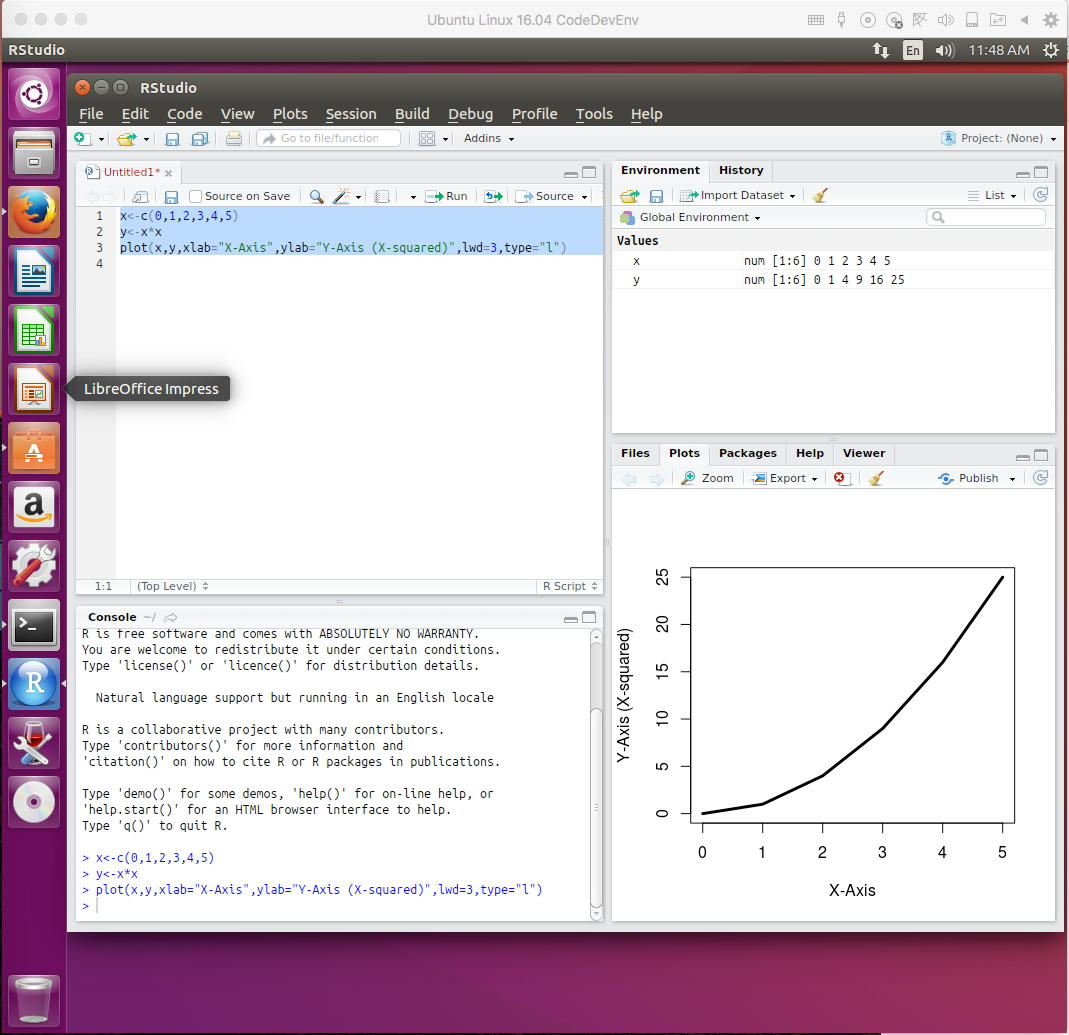
\includegraphics[width=4.5in]{./1-Introduction/LinuxRStudioCompleted.jpg} 
   \caption{Completed script run.  Notice the plot in the lower right panel.  At this point you have a functioning programming tool}
   \label{fig:LinuxRStudioCompleted}
\end{figure}

\clearpage

%\subsection{Exercises}

%%%%%%%%%%%%%%%%%%%%%%%%%%%%%%%%%%%%%%%%%%%%%%%%%%%%%%%%%%%%%%